\documentclass[twoside]{book}

% Packages required by doxygen
\usepackage{calc}
\usepackage{doxygen}
\usepackage{graphicx}
\usepackage[utf8]{inputenc}
\usepackage{makeidx}
\usepackage{multicol}
\usepackage{multirow}
\usepackage{fixltx2e}
\PassOptionsToPackage{warn}{textcomp}
\usepackage{textcomp}
\usepackage[nointegrals]{wasysym}
\usepackage[table]{xcolor}

% Font selection
\usepackage[T1]{fontenc}
\usepackage{mathptmx}
\usepackage[scaled=.90]{helvet}
\usepackage{courier}
\usepackage{amssymb}
\usepackage{sectsty}
\renewcommand{\familydefault}{\sfdefault}
\allsectionsfont{%
  \fontseries{bc}\selectfont%
  \color{darkgray}%
}
\renewcommand{\DoxyLabelFont}{%
  \fontseries{bc}\selectfont%
  \color{darkgray}%
}
\newcommand{\+}{\discretionary{\mbox{\scriptsize$\hookleftarrow$}}{}{}}

% Page & text layout
\usepackage{geometry}
\geometry{%
  a4paper,%
  top=2.5cm,%
  bottom=2.5cm,%
  left=2.5cm,%
  right=2.5cm%
}
\tolerance=750
\hfuzz=15pt
\hbadness=750
\setlength{\emergencystretch}{15pt}
\setlength{\parindent}{0cm}
\setlength{\parskip}{0.2cm}
\makeatletter
\renewcommand{\paragraph}{%
  \@startsection{paragraph}{4}{0ex}{-1.0ex}{1.0ex}{%
    \normalfont\normalsize\bfseries\SS@parafont%
  }%
}
\renewcommand{\subparagraph}{%
  \@startsection{subparagraph}{5}{0ex}{-1.0ex}{1.0ex}{%
    \normalfont\normalsize\bfseries\SS@subparafont%
  }%
}
\makeatother

% Headers & footers
\usepackage{fancyhdr}
\pagestyle{fancyplain}
\fancyhead[LE]{\fancyplain{}{\bfseries\thepage}}
\fancyhead[CE]{\fancyplain{}{}}
\fancyhead[RE]{\fancyplain{}{\bfseries\leftmark}}
\fancyhead[LO]{\fancyplain{}{\bfseries\rightmark}}
\fancyhead[CO]{\fancyplain{}{}}
\fancyhead[RO]{\fancyplain{}{\bfseries\thepage}}
\fancyfoot[LE]{\fancyplain{}{}}
\fancyfoot[CE]{\fancyplain{}{}}
\fancyfoot[RE]{\fancyplain{}{\bfseries\scriptsize Generated on Mon Aug 18 2014 16\+:58\+:44 for T\+K\+R\+T\+A\+P by Doxygen }}
\fancyfoot[LO]{\fancyplain{}{\bfseries\scriptsize Generated on Mon Aug 18 2014 16\+:58\+:44 for T\+K\+R\+T\+A\+P by Doxygen }}
\fancyfoot[CO]{\fancyplain{}{}}
\fancyfoot[RO]{\fancyplain{}{}}
\renewcommand{\footrulewidth}{0.4pt}
\renewcommand{\chaptermark}[1]{%
  \markboth{#1}{}%
}
\renewcommand{\sectionmark}[1]{%
  \markright{\thesection\ #1}%
}

% Indices & bibliography
\usepackage{natbib}
\usepackage[titles]{tocloft}
\setcounter{tocdepth}{3}
\setcounter{secnumdepth}{5}
\makeindex

% Hyperlinks (required, but should be loaded last)
\usepackage{ifpdf}
\ifpdf
  \usepackage[pdftex,pagebackref=true]{hyperref}
\else
  \usepackage[ps2pdf,pagebackref=true]{hyperref}
\fi
\hypersetup{%
  colorlinks=true,%
  linkcolor=blue,%
  citecolor=blue,%
  unicode%
}

% Custom commands
\newcommand{\clearemptydoublepage}{%
  \newpage{\pagestyle{empty}\cleardoublepage}%
}


%===== C O N T E N T S =====

\begin{document}

% Titlepage & ToC
\hypersetup{pageanchor=false,
             bookmarks=true,
             bookmarksnumbered=true,
             pdfencoding=unicode
            }
\pagenumbering{roman}
\begin{titlepage}
\vspace*{7cm}
\begin{center}%
{\Large T\+K\+R\+T\+A\+P \\[1ex]\large 1.\+0.\+0 }\\
\vspace*{1cm}
{\large Generated by Doxygen 1.8.7}\\
\vspace*{0.5cm}
{\small Mon Aug 18 2014 16:58:44}\\
\end{center}
\end{titlepage}
\clearemptydoublepage
\tableofcontents
\clearemptydoublepage
\pagenumbering{arabic}
\hypersetup{pageanchor=true}

%--- Begin generated contents ---
\chapter{T\+K\+R\+T\+A\+P}
\label{md__c_1__users__q__documents__git_hub__t_k_r_t_a_p__r_e_a_d_m_e}
\hypertarget{md__c_1__users__q__documents__git_hub__t_k_r_t_a_p__r_e_a_d_m_e}{}
\hyperlink{class_t_k_r_t_a_p}{T\+K\+R\+T\+A\+P} U\+I Program 
\chapter{Hierarchical Index}
\section{Class Hierarchy}
This inheritance list is sorted roughly, but not completely, alphabetically\+:\begin{DoxyCompactList}
\item Q\+Dialog\begin{DoxyCompactList}
\item \contentsline{section}{Market\+Map\+View}{\pageref{class_market_map_view}}{}
\item \contentsline{section}{Quick\+Stock\+Chart}{\pageref{class_quick_stock_chart}}{}
\end{DoxyCompactList}
\item Q\+Main\+Window\begin{DoxyCompactList}
\item \contentsline{section}{T\+K\+R\+T\+A\+P}{\pageref{class_t_k_r_t_a_p}}{}
\end{DoxyCompactList}
\item Q\+Object\begin{DoxyCompactList}
\item \contentsline{section}{Json\+Query}{\pageref{class_json_query}}{}
\item \contentsline{section}{Matrice\+Rgb}{\pageref{class_matrice_rgb}}{}
\item \contentsline{section}{Rss\+Client}{\pageref{class_rss_client}}{}
\end{DoxyCompactList}
\end{DoxyCompactList}

\chapter{Class Index}
\section{Class List}
Here are the classes, structs, unions and interfaces with brief descriptions\+:\begin{DoxyCompactList}
\item\contentsline{section}{\hyperlink{class_json_query}{Json\+Query} \\*Handles the J\+S\+O\+N queries to Quandl and Yahoo and parses them into a simple string }{\pageref{class_json_query}}{}
\item\contentsline{section}{\hyperlink{class_market_map_view}{Market\+Map\+View} }{\pageref{class_market_map_view}}{}
\item\contentsline{section}{\hyperlink{class_matrice_rgb}{Matrice\+Rgb} \\*Used to link the physical matrix display with the rest of the program. It can write text on both lines of the display in 8 different colours }{\pageref{class_matrice_rgb}}{}
\item\contentsline{section}{\hyperlink{class_quick_stock_chart}{Quick\+Stock\+Chart} }{\pageref{class_quick_stock_chart}}{}
\item\contentsline{section}{\hyperlink{class_rss_client}{Rss\+Client} \\*Handles the reception and sorting (by date) of multiple R\+S\+S news feeds }{\pageref{class_rss_client}}{}
\item\contentsline{section}{\hyperlink{class_t_k_r_t_a_p}{T\+K\+R\+T\+A\+P} }{\pageref{class_t_k_r_t_a_p}}{}
\end{DoxyCompactList}

\chapter{File Index}
\section{File List}
Here is a list of all documented files with brief descriptions\+:\begin{DoxyCompactList}
\item\contentsline{section}{C\+:/\+Users/\+Q/\+Documents/\+Git\+Hub/\+T\+K\+R\+T\+A\+P/\hyperlink{jsonquery_8cpp}{jsonquery.\+cpp} \\*Implementation of the jsonquery class }{\pageref{jsonquery_8cpp}}{}
\item\contentsline{section}{C\+:/\+Users/\+Q/\+Documents/\+Git\+Hub/\+T\+K\+R\+T\+A\+P/\hyperlink{jsonquery_8h}{jsonquery.\+h} \\*Implementation of the jsonquery class }{\pageref{jsonquery_8h}}{}
\item\contentsline{section}{C\+:/\+Users/\+Q/\+Documents/\+Git\+Hub/\+T\+K\+R\+T\+A\+P/\hyperlink{main_8cpp}{main.\+cpp} \\*Implementation of the main G\+U\+I class }{\pageref{main_8cpp}}{}
\item\contentsline{section}{C\+:/\+Users/\+Q/\+Documents/\+Git\+Hub/\+T\+K\+R\+T\+A\+P/\hyperlink{marketmapview_8cpp}{marketmapview.\+cpp} \\*Implementation of the Market Map dialog window }{\pageref{marketmapview_8cpp}}{}
\item\contentsline{section}{C\+:/\+Users/\+Q/\+Documents/\+Git\+Hub/\+T\+K\+R\+T\+A\+P/\hyperlink{marketmapview_8h}{marketmapview.\+h} \\*Implementation of the Market Map dialog window }{\pageref{marketmapview_8h}}{}
\item\contentsline{section}{C\+:/\+Users/\+Q/\+Documents/\+Git\+Hub/\+T\+K\+R\+T\+A\+P/\hyperlink{matricergb_8cpp}{matricergb.\+cpp} \\*Implementation of the R\+G\+B Matrix class }{\pageref{matricergb_8cpp}}{}
\item\contentsline{section}{C\+:/\+Users/\+Q/\+Documents/\+Git\+Hub/\+T\+K\+R\+T\+A\+P/\hyperlink{matricergb_8h}{matricergb.\+h} \\*Declaration of the R\+G\+B Matrix class }{\pageref{matricergb_8h}}{}
\item\contentsline{section}{C\+:/\+Users/\+Q/\+Documents/\+Git\+Hub/\+T\+K\+R\+T\+A\+P/\hyperlink{quickstockchart_8cpp}{quickstockchart.\+cpp} \\*Implementation of the stock chart dialog window }{\pageref{quickstockchart_8cpp}}{}
\item\contentsline{section}{C\+:/\+Users/\+Q/\+Documents/\+Git\+Hub/\+T\+K\+R\+T\+A\+P/\hyperlink{quickstockchart_8h}{quickstockchart.\+h} \\*Implementation of the stock chart dialog window }{\pageref{quickstockchart_8h}}{}
\item\contentsline{section}{C\+:/\+Users/\+Q/\+Documents/\+Git\+Hub/\+T\+K\+R\+T\+A\+P/\hyperlink{rssclient_8cpp}{rssclient.\+cpp} \\*Implementation of the R\+S\+S client class }{\pageref{rssclient_8cpp}}{}
\item\contentsline{section}{C\+:/\+Users/\+Q/\+Documents/\+Git\+Hub/\+T\+K\+R\+T\+A\+P/\hyperlink{rssclient_8h}{rssclient.\+h} \\*Implementation of the R\+S\+S client class }{\pageref{rssclient_8h}}{}
\item\contentsline{section}{C\+:/\+Users/\+Q/\+Documents/\+Git\+Hub/\+T\+K\+R\+T\+A\+P/\hyperlink{tkrtap_8cpp}{tkrtap.\+cpp} \\*Implementation of the main G\+U\+I class }{\pageref{tkrtap_8cpp}}{}
\item\contentsline{section}{C\+:/\+Users/\+Q/\+Documents/\+Git\+Hub/\+T\+K\+R\+T\+A\+P/\hyperlink{tkrtap_8h}{tkrtap.\+h} \\*Implementation of the main G\+U\+I class }{\pageref{tkrtap_8h}}{}
\end{DoxyCompactList}

\chapter{Class Documentation}
\hypertarget{class_json_query}{\section{Json\+Query Class Reference}
\label{class_json_query}\index{Json\+Query@{Json\+Query}}
}


The \hyperlink{class_json_query}{Json\+Query} class handles the J\+S\+O\+N queries to Quandl and Yahoo and parses them into a simple string.  




{\ttfamily \#include $<$jsonquery.\+h$>$}

Inheritance diagram for Json\+Query\+:\begin{figure}[H]
\begin{center}
\leavevmode
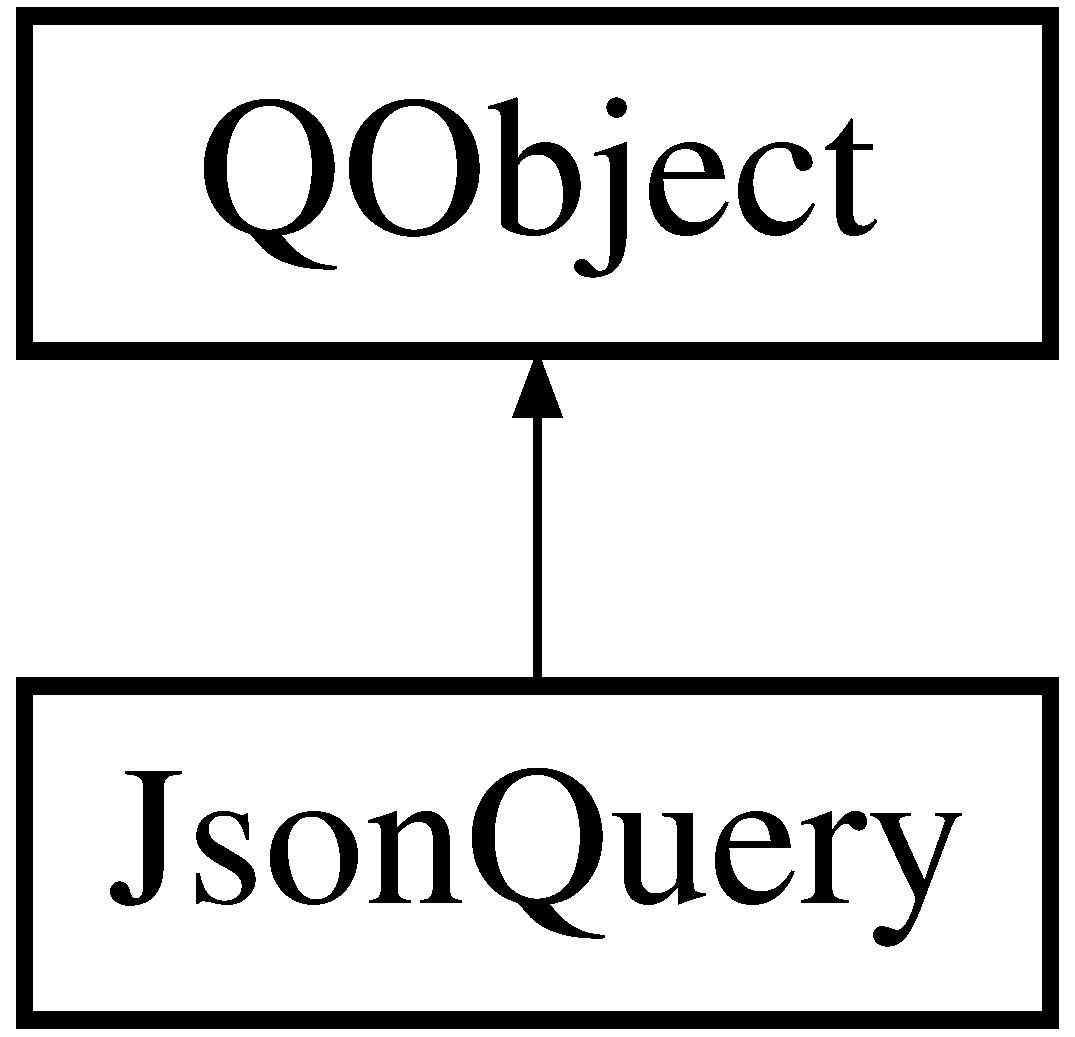
\includegraphics[height=2.000000cm]{class_json_query}
\end{center}
\end{figure}
\subsection*{Public Slots}
\begin{DoxyCompactItemize}
\item 
\hypertarget{class_json_query_a7ac6e8248b34fec56a6cfadee48ff867}{void \hyperlink{class_json_query_a7ac6e8248b34fec56a6cfadee48ff867}{send\+Request} ()}\label{class_json_query_a7ac6e8248b34fec56a6cfadee48ff867}

\begin{DoxyCompactList}\small\item\em Sets up the request and connects the proper signal to the parsing function. \end{DoxyCompactList}\end{DoxyCompactItemize}
\subsection*{Signals}
\begin{DoxyCompactItemize}
\item 
void \hyperlink{class_json_query_a384e9fd610b9046695a1f1f12e7e3ba6}{parsing\+Complete} (Q\+String\+List str\+\_\+list, Q\+String str\+\_\+colour)
\begin{DoxyCompactList}\small\item\em Signal used when the J\+S\+O\+N request has been parsed. \end{DoxyCompactList}\end{DoxyCompactItemize}
\subsection*{Public Member Functions}
\begin{DoxyCompactItemize}
\item 
\hyperlink{class_json_query_a8ea4951a7e633564dd0b3fa09dc9ddec}{Json\+Query} (Q\+Object $\ast$parent=0)
\begin{DoxyCompactList}\small\item\em Default constructor. \end{DoxyCompactList}\item 
void \hyperlink{class_json_query_a173751689d3ecc26d34a2673b83191f6}{set\+Service\+Name} (Q\+String service\+\_\+name)
\begin{DoxyCompactList}\small\item\em Sets the service used for the J\+S\+O\+N query. \end{DoxyCompactList}\item 
void \hyperlink{class_json_query_a79acc90e20082bdfc6ab72a4c2444b26}{set\+Ticker\+Names} (Q\+String\+List tkr\+\_\+names)
\begin{DoxyCompactList}\small\item\em Sets the list of tickers. \end{DoxyCompactList}\item 
void \hyperlink{class_json_query_afefa6f2e54d664970c0b4ba1d041606c}{set\+Auth\+Code\+Quandl} (Q\+String aut\+\_\+code)
\begin{DoxyCompactList}\small\item\em Set the Quandl auth code. \end{DoxyCompactList}\end{DoxyCompactItemize}
\subsection*{Private Slots}
\begin{DoxyCompactItemize}
\item 
\hypertarget{class_json_query_ad6bddcda7bd4af909e45bd2ca392b275}{void \hyperlink{class_json_query_ad6bddcda7bd4af909e45bd2ca392b275}{parse\+J\+S\+O\+N} ()}\label{class_json_query_ad6bddcda7bd4af909e45bd2ca392b275}

\begin{DoxyCompactList}\small\item\em Parses the received information from the J\+S\+O\+N request and emits the \hyperlink{class_json_query_a384e9fd610b9046695a1f1f12e7e3ba6}{parsing\+Complete()} signal when done. \end{DoxyCompactList}\end{DoxyCompactItemize}
\subsection*{Private Member Functions}
\begin{DoxyCompactItemize}
\item 
Q\+Url \hyperlink{class_json_query_adc17cbbe26433d97421ea81fb873b2f0}{create\+Json\+Url} ()
\begin{DoxyCompactList}\small\item\em Creates an U\+R\+L using the ticker names for Quandl or Yahoo. \end{DoxyCompactList}\end{DoxyCompactItemize}
\subsection*{Private Attributes}
\begin{DoxyCompactItemize}
\item 
\hypertarget{class_json_query_acc3c7eca201fdc8e1ebc5d1f8763631c}{Q\+String \hyperlink{class_json_query_acc3c7eca201fdc8e1ebc5d1f8763631c}{\+\_\+service\+\_\+name}}\label{class_json_query_acc3c7eca201fdc8e1ebc5d1f8763631c}

\begin{DoxyCompactList}\small\item\em The name of the J\+S\+O\+N data service provider. Note\+: Only Quandl and Yahoo are currently supported. \end{DoxyCompactList}\item 
\hypertarget{class_json_query_adf76972f9f175db206bb842fc73e7913}{Q\+String\+List \hyperlink{class_json_query_adf76972f9f175db206bb842fc73e7913}{\+\_\+ticker\+\_\+names}}\label{class_json_query_adf76972f9f175db206bb842fc73e7913}

\begin{DoxyCompactList}\small\item\em List of tickers. \end{DoxyCompactList}\item 
\hypertarget{class_json_query_a9f7f1c04e4e659e94046eafb7c9d65a9}{Q\+String \hyperlink{class_json_query_a9f7f1c04e4e659e94046eafb7c9d65a9}{\+\_\+\+Quandl\+\_\+auth\+\_\+token}}\label{class_json_query_a9f7f1c04e4e659e94046eafb7c9d65a9}

\begin{DoxyCompactList}\small\item\em The Quandl Auth token is needed to make more than 50 requests per day. \end{DoxyCompactList}\item 
\hypertarget{class_json_query_a6a656b6284308e14c88cd2f325d3f82d}{Q\+Network\+Access\+Manager \hyperlink{class_json_query_a6a656b6284308e14c88cd2f325d3f82d}{\+\_\+manager}}\label{class_json_query_a6a656b6284308e14c88cd2f325d3f82d}

\begin{DoxyCompactList}\small\item\em The Network manager used to send the J\+S\+O\+N requests. \end{DoxyCompactList}\item 
\hypertarget{class_json_query_a421d1210dc3918200f4b2fad77f98726}{Q\+Network\+Reply $\ast$ \hyperlink{class_json_query_a421d1210dc3918200f4b2fad77f98726}{\+\_\+current\+\_\+reply}}\label{class_json_query_a421d1210dc3918200f4b2fad77f98726}

\begin{DoxyCompactList}\small\item\em The current reply. \end{DoxyCompactList}\end{DoxyCompactItemize}


\subsection{Detailed Description}
The \hyperlink{class_json_query}{Json\+Query} class handles the J\+S\+O\+N queries to Quandl and Yahoo and parses them into a simple string. 

\subsection{Constructor \& Destructor Documentation}
\hypertarget{class_json_query_a8ea4951a7e633564dd0b3fa09dc9ddec}{\index{Json\+Query@{Json\+Query}!Json\+Query@{Json\+Query}}
\index{Json\+Query@{Json\+Query}!Json\+Query@{Json\+Query}}
\subsubsection[{Json\+Query}]{\setlength{\rightskip}{0pt plus 5cm}Json\+Query\+::\+Json\+Query (
\begin{DoxyParamCaption}
\item[{Q\+Object $\ast$}]{parent = {\ttfamily 0}}
\end{DoxyParamCaption}
)\hspace{0.3cm}{\ttfamily [explicit]}}}\label{class_json_query_a8ea4951a7e633564dd0b3fa09dc9ddec}


Default constructor. 


\begin{DoxyParams}{Parameters}
{\em parent} & Parent of the object (default = 0) \\
\hline
\end{DoxyParams}


\subsection{Member Function Documentation}
\hypertarget{class_json_query_adc17cbbe26433d97421ea81fb873b2f0}{\index{Json\+Query@{Json\+Query}!create\+Json\+Url@{create\+Json\+Url}}
\index{create\+Json\+Url@{create\+Json\+Url}!Json\+Query@{Json\+Query}}
\subsubsection[{create\+Json\+Url}]{\setlength{\rightskip}{0pt plus 5cm}Q\+Url Json\+Query\+::create\+Json\+Url (
\begin{DoxyParamCaption}
{}
\end{DoxyParamCaption}
)\hspace{0.3cm}{\ttfamily [private]}}}\label{class_json_query_adc17cbbe26433d97421ea81fb873b2f0}


Creates an U\+R\+L using the ticker names for Quandl or Yahoo. 

\begin{DoxyReturn}{Returns}
The Q\+Url for the specified J\+S\+O\+N request 
\end{DoxyReturn}
\hypertarget{class_json_query_a384e9fd610b9046695a1f1f12e7e3ba6}{\index{Json\+Query@{Json\+Query}!parsing\+Complete@{parsing\+Complete}}
\index{parsing\+Complete@{parsing\+Complete}!Json\+Query@{Json\+Query}}
\subsubsection[{parsing\+Complete}]{\setlength{\rightskip}{0pt plus 5cm}void Json\+Query\+::parsing\+Complete (
\begin{DoxyParamCaption}
\item[{Q\+String\+List}]{str\+\_\+list, }
\item[{Q\+String}]{str\+\_\+colour}
\end{DoxyParamCaption}
)\hspace{0.3cm}{\ttfamily [signal]}}}\label{class_json_query_a384e9fd610b9046695a1f1f12e7e3ba6}


Signal used when the J\+S\+O\+N request has been parsed. 


\begin{DoxyParams}{Parameters}
{\em str\+\_\+list} & The formatted text message String List \\
\hline
{\em str\+\_\+colour} & The formatted colour string \\
\hline
\end{DoxyParams}
\hypertarget{class_json_query_afefa6f2e54d664970c0b4ba1d041606c}{\index{Json\+Query@{Json\+Query}!set\+Auth\+Code\+Quandl@{set\+Auth\+Code\+Quandl}}
\index{set\+Auth\+Code\+Quandl@{set\+Auth\+Code\+Quandl}!Json\+Query@{Json\+Query}}
\subsubsection[{set\+Auth\+Code\+Quandl}]{\setlength{\rightskip}{0pt plus 5cm}void Json\+Query\+::set\+Auth\+Code\+Quandl (
\begin{DoxyParamCaption}
\item[{Q\+String}]{auth\+\_\+code}
\end{DoxyParamCaption}
)\hspace{0.3cm}{\ttfamily [inline]}}}\label{class_json_query_afefa6f2e54d664970c0b4ba1d041606c}


Set the Quandl auth code. 


\begin{DoxyParams}{Parameters}
{\em auth\+\_\+code} & The auth code used by Quandl \\
\hline
\end{DoxyParams}
\hypertarget{class_json_query_a173751689d3ecc26d34a2673b83191f6}{\index{Json\+Query@{Json\+Query}!set\+Service\+Name@{set\+Service\+Name}}
\index{set\+Service\+Name@{set\+Service\+Name}!Json\+Query@{Json\+Query}}
\subsubsection[{set\+Service\+Name}]{\setlength{\rightskip}{0pt plus 5cm}void Json\+Query\+::set\+Service\+Name (
\begin{DoxyParamCaption}
\item[{Q\+String}]{service\+\_\+name}
\end{DoxyParamCaption}
)\hspace{0.3cm}{\ttfamily [inline]}}}\label{class_json_query_a173751689d3ecc26d34a2673b83191f6}


Sets the service used for the J\+S\+O\+N query. 


\begin{DoxyParams}{Parameters}
{\em service\+\_\+name} & The name of the chosen service \\
\hline
\end{DoxyParams}
\hypertarget{class_json_query_a79acc90e20082bdfc6ab72a4c2444b26}{\index{Json\+Query@{Json\+Query}!set\+Ticker\+Names@{set\+Ticker\+Names}}
\index{set\+Ticker\+Names@{set\+Ticker\+Names}!Json\+Query@{Json\+Query}}
\subsubsection[{set\+Ticker\+Names}]{\setlength{\rightskip}{0pt plus 5cm}void Json\+Query\+::set\+Ticker\+Names (
\begin{DoxyParamCaption}
\item[{Q\+String\+List}]{tkr\+\_\+names}
\end{DoxyParamCaption}
)\hspace{0.3cm}{\ttfamily [inline]}}}\label{class_json_query_a79acc90e20082bdfc6ab72a4c2444b26}


Sets the list of tickers. 


\begin{DoxyParams}{Parameters}
{\em tkr\+\_\+names} & The list of tickers \\
\hline
\end{DoxyParams}


The documentation for this class was generated from the following files\+:\begin{DoxyCompactItemize}
\item 
C\+:/\+Users/\+Q/\+Documents/\+Git\+Hub/\+T\+K\+R\+T\+A\+P/\hyperlink{jsonquery_8h}{jsonquery.\+h}\item 
C\+:/\+Users/\+Q/\+Documents/\+Git\+Hub/\+T\+K\+R\+T\+A\+P/\hyperlink{jsonquery_8cpp}{jsonquery.\+cpp}\end{DoxyCompactItemize}

\hypertarget{class_market_map_view}{\section{Market\+Map\+View Class Reference}
\label{class_market_map_view}\index{Market\+Map\+View@{Market\+Map\+View}}
}
Inheritance diagram for Market\+Map\+View\+:\begin{figure}[H]
\begin{center}
\leavevmode
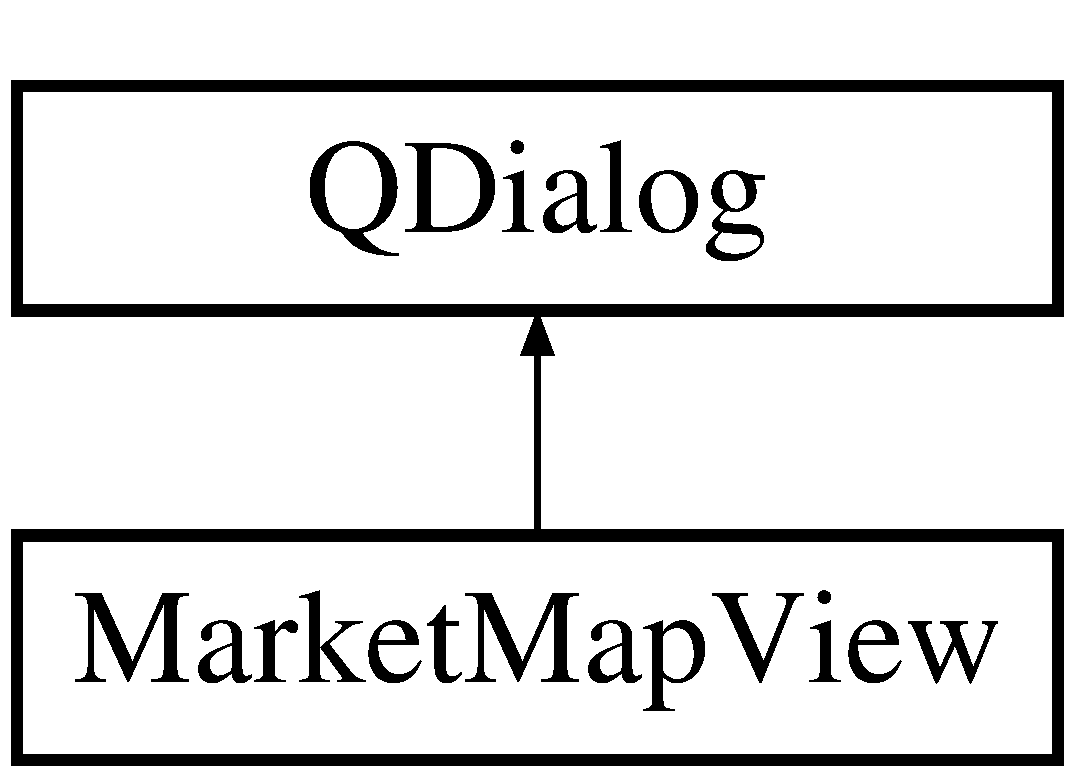
\includegraphics[height=2.000000cm]{class_market_map_view}
\end{center}
\end{figure}
\subsection*{Public Member Functions}
\begin{DoxyCompactItemize}
\item 
\hypertarget{class_market_map_view_ad68b944d6f3ef350a1d6925b2f974a90}{{\bfseries Market\+Map\+View} (Q\+Widget $\ast$parent=0, Q\+Url Map\+Url=Q\+Url(\char`\"{}http\+://www.\+finviz.\+com/map.\+ashx?t=sec\char`\"{}))}\label{class_market_map_view_ad68b944d6f3ef350a1d6925b2f974a90}

\end{DoxyCompactItemize}
\subsection*{Private Slots}
\begin{DoxyCompactItemize}
\item 
\hypertarget{class_market_map_view_ae680dd9e4cffd99085ce9d0aecaebd0c}{void {\bfseries save\+Position} ()}\label{class_market_map_view_ae680dd9e4cffd99085ce9d0aecaebd0c}

\item 
\hypertarget{class_market_map_view_a5bf3380427a2fca3737acff9c0e82bf2}{void {\bfseries load\+Position} ()}\label{class_market_map_view_a5bf3380427a2fca3737acff9c0e82bf2}

\item 
\hypertarget{class_market_map_view_aeb74298240bbc6d4af02e06c3cc8aa79}{void {\bfseries close\+Event} (Q\+Close\+Event $\ast$event)}\label{class_market_map_view_aeb74298240bbc6d4af02e06c3cc8aa79}

\end{DoxyCompactItemize}
\subsection*{Private Attributes}
\begin{DoxyCompactItemize}
\item 
\hypertarget{class_market_map_view_ad147de5cb234034d0140aa3ba132d49b}{Ui\+::\+Market\+Map\+View $\ast$ {\bfseries ui}}\label{class_market_map_view_ad147de5cb234034d0140aa3ba132d49b}

\end{DoxyCompactItemize}


The documentation for this class was generated from the following files\+:\begin{DoxyCompactItemize}
\item 
C\+:/\+Users/\+Q/\+Documents/\+Git\+Hub/\+T\+K\+R\+T\+A\+P/\hyperlink{marketmapview_8h}{marketmapview.\+h}\item 
C\+:/\+Users/\+Q/\+Documents/\+Git\+Hub/\+T\+K\+R\+T\+A\+P/\hyperlink{marketmapview_8cpp}{marketmapview.\+cpp}\end{DoxyCompactItemize}

\hypertarget{class_matrice_rgb}{\section{Matrice\+Rgb Class Reference}
\label{class_matrice_rgb}\index{Matrice\+Rgb@{Matrice\+Rgb}}
}


The \hyperlink{class_matrice_rgb}{Matrice\+Rgb} class is used to link the physical matrix display with the rest of the program. It can write text on both lines of the display in 8 different colours.  




{\ttfamily \#include $<$matricergb.\+h$>$}

Inheritance diagram for Matrice\+Rgb\+:\begin{figure}[H]
\begin{center}
\leavevmode
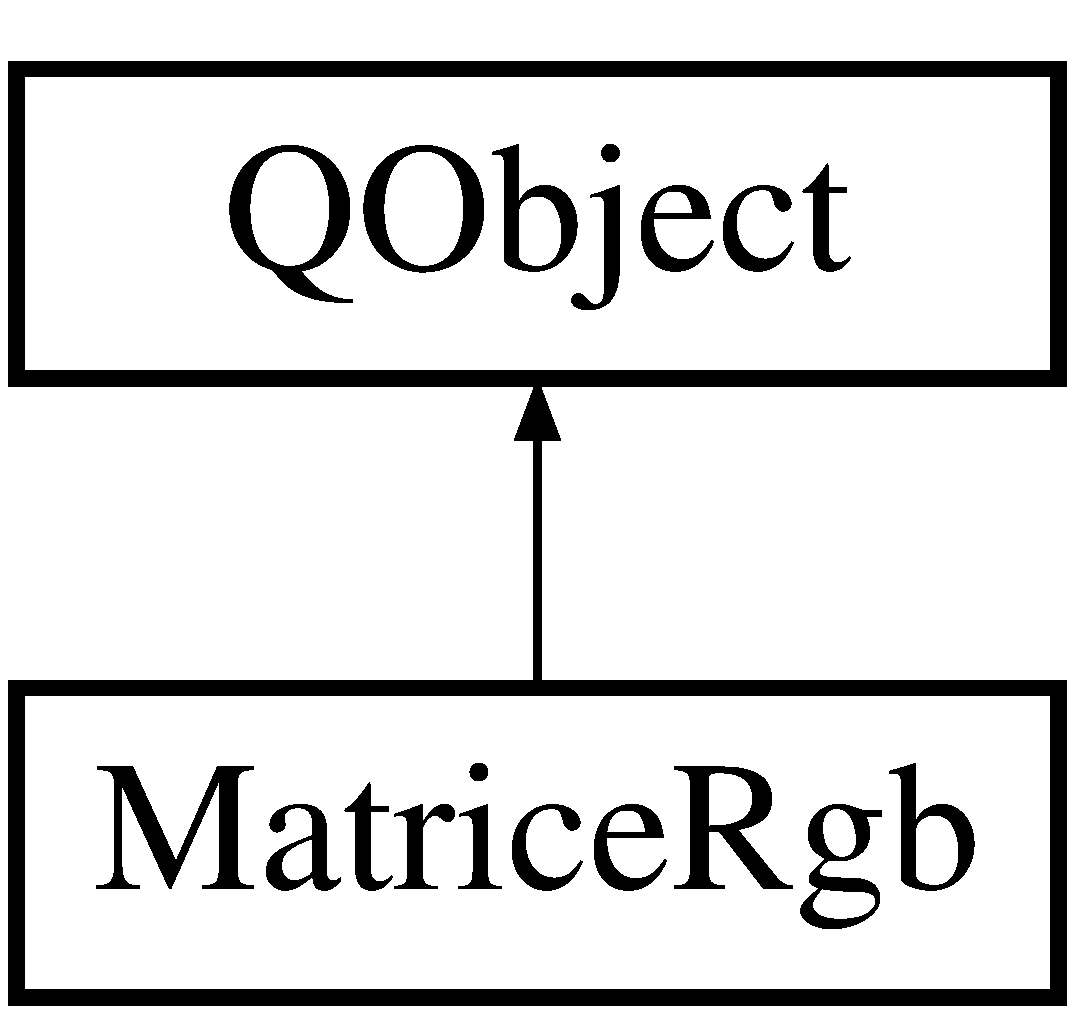
\includegraphics[height=2.000000cm]{class_matrice_rgb}
\end{center}
\end{figure}
\subsection*{Public Slots}
\begin{DoxyCompactItemize}
\item 
void \hyperlink{class_matrice_rgb_abb55a1dd2c309df8694474dc45b00312}{set\+Port\+Name} (Q\+String nom\+\_\+port)
\begin{DoxyCompactList}\small\item\em Sets the serial port that will be used. \end{DoxyCompactList}\item 
bool \hyperlink{class_matrice_rgb_a8afdf4dd08a76e5dec012145ccff96e9}{toggle\+Serial\+Port} ()
\begin{DoxyCompactList}\small\item\em Toggles the chosen serial port O\+N/\+O\+F\+F. Will pass any O\+S error through an error dialog. \end{DoxyCompactList}\item 
\hypertarget{class_matrice_rgb_a5cdc2dbbf78aab29dc654860b49a0891}{void \hyperlink{class_matrice_rgb_a5cdc2dbbf78aab29dc654860b49a0891}{send\+All} ()}\label{class_matrice_rgb_a5cdc2dbbf78aab29dc654860b49a0891}

\begin{DoxyCompactList}\small\item\em Sends the text and colour information for both lines of the matrix. \end{DoxyCompactList}\item 
void \hyperlink{class_matrice_rgb_aa130211f4d06d132699015a6bc6f3382}{send\+Line} (int line\+\_\+no)
\begin{DoxyCompactList}\small\item\em Sends the text and color information of one line to the matrix over the serial port. \end{DoxyCompactList}\item 
void \hyperlink{class_matrice_rgb_aaf9c466a7ddbe850730fed54e951078f}{send\+Speed} (unsigned char speed=15)
\begin{DoxyCompactList}\small\item\em Sends the scroll speed (in ms) to the display. Default is 15ms. \end{DoxyCompactList}\end{DoxyCompactItemize}
\subsection*{Public Member Functions}
\begin{DoxyCompactItemize}
\item 
\hypertarget{class_matrice_rgb_aea79aaf12329d33f4f0d5f06d15929a6}{\hyperlink{class_matrice_rgb_aea79aaf12329d33f4f0d5f06d15929a6}{Matrice\+Rgb} ()}\label{class_matrice_rgb_aea79aaf12329d33f4f0d5f06d15929a6}

\begin{DoxyCompactList}\small\item\em Default constuctor This constructor does not need any parameters. \end{DoxyCompactList}\item 
void \hyperlink{class_matrice_rgb_a2e60d3e1608cf676b597aa3bbe7ffbe7}{set\+Text} (Q\+String txt\+\_\+line, int line\+\_\+no)
\begin{DoxyCompactList}\small\item\em Sets the text for a given line. \end{DoxyCompactList}\item 
void \hyperlink{class_matrice_rgb_aaf8facb904df841ef6f22a842715a2b9}{set\+String\+Color} (Q\+String txt\+\_\+colour, int line\+\_\+no)
\begin{DoxyCompactList}\small\item\em Sets the colour string for the specified line. \end{DoxyCompactList}\item 
void \hyperlink{class_matrice_rgb_ad7ed9e4715ed21491f33b3db48f5d436}{set\+Default\+Colors} (int $\ast$colours)
\begin{DoxyCompactList}\small\item\em Sets the default colour information. \end{DoxyCompactList}\item 
Q\+List$<$ Q\+Serial\+Port\+Info $>$ \hyperlink{class_matrice_rgb_a49199cd529e603db49cffd85b813e49a}{get\+List\+Ports} ()
\begin{DoxyCompactList}\small\item\em Returns a Q\+List of the available serial ports as returned by the O\+S. This is a list of Q\+Serial\+Port\+Info. \end{DoxyCompactList}\end{DoxyCompactItemize}
\subsection*{Private Member Functions}
\begin{DoxyCompactItemize}
\item 
Q\+String \hyperlink{class_matrice_rgb_a53a4ee970396d25468dd263d4bede177}{unicodeto\+C\+P437} (Q\+String unicode\+\_\+str)
\begin{DoxyCompactList}\small\item\em Converts a Unicode Q\+String to a slightly modified version of the C\+P437 \char`\"{}standard\char`\"{} that is used in the physical matrix's R\+O\+M. The matrix uses a slightly modified version of the \href{http://en.wikipedia.org/wiki/Cp437}{\tt C\+P437} character set. \end{DoxyCompactList}\item 
Q\+String \hyperlink{class_matrice_rgb_a05ea8eaf536cc656dfe993710221aa30}{create\+Color\+String} (int line\+\_\+no)
\begin{DoxyCompactList}\small\item\em Creates a color string using the default parameters. \end{DoxyCompactList}\item 
unsigned char \hyperlink{class_matrice_rgb_ab3067fe6615c058957d51f345ab2dba6}{calcul\+C\+R\+C} (const char $\ast$message, int length)
\begin{DoxyCompactList}\small\item\em Calculates a simple C\+R\+C8 on a char array. This code was taken from \href{http://www.leonardomiliani.com/en/2013/un-semplice-crc8-per-arduino/}{\tt here}. \end{DoxyCompactList}\end{DoxyCompactItemize}
\subsection*{Private Attributes}
\begin{DoxyCompactItemize}
\item 
\hypertarget{class_matrice_rgb_a4593df682e52dceeeb40cc10da8f7d19}{unsigned char \hyperlink{class_matrice_rgb_a4593df682e52dceeeb40cc10da8f7d19}{\+\_\+scroll\+\_\+speed}}\label{class_matrice_rgb_a4593df682e52dceeeb40cc10da8f7d19}

\begin{DoxyCompactList}\small\item\em The Scroll speed of the message in ms. \end{DoxyCompactList}\item 
\hypertarget{class_matrice_rgb_a3e30ec8b0b50ea4eb417cba8b2b1ce20}{int \hyperlink{class_matrice_rgb_a3e30ec8b0b50ea4eb417cba8b2b1ce20}{\+\_\+number\+\_\+of\+\_\+led\+\_\+matrices}}\label{class_matrice_rgb_a3e30ec8b0b50ea4eb417cba8b2b1ce20}

\begin{DoxyCompactList}\small\item\em The number of L\+E\+D matrices on the display. \end{DoxyCompactList}\item 
\hypertarget{class_matrice_rgb_abec209cc567ab2b491f1b65140f2e9a1}{Q\+Serial\+Port $\ast$ \hyperlink{class_matrice_rgb_abec209cc567ab2b491f1b65140f2e9a1}{\+\_\+serial}}\label{class_matrice_rgb_abec209cc567ab2b491f1b65140f2e9a1}

\begin{DoxyCompactList}\small\item\em Pointer to a Q\+Serial\+Port object. \end{DoxyCompactList}\item 
\hypertarget{class_matrice_rgb_a43eefbe8adeec9f8b899aa9957a769a9}{Q\+String \hyperlink{class_matrice_rgb_a43eefbe8adeec9f8b899aa9957a769a9}{\+\_\+string\+\_\+lines} \mbox{[}2\mbox{]}}\label{class_matrice_rgb_a43eefbe8adeec9f8b899aa9957a769a9}

\begin{DoxyCompactList}\small\item\em The array of Q\+Strings containing the message's text. \end{DoxyCompactList}\item 
\hypertarget{class_matrice_rgb_a7bf7a29cbec11d90407df759baf888fd}{Q\+String \hyperlink{class_matrice_rgb_a7bf7a29cbec11d90407df759baf888fd}{\+\_\+string\+\_\+colours} \mbox{[}2\mbox{]}}\label{class_matrice_rgb_a7bf7a29cbec11d90407df759baf888fd}

\begin{DoxyCompactList}\small\item\em The array of Q\+String containing the message's colour information. \end{DoxyCompactList}\item 
\hypertarget{class_matrice_rgb_a8298c7c9169743e9118e39e1d87edc8e}{Q\+String \hyperlink{class_matrice_rgb_a8298c7c9169743e9118e39e1d87edc8e}{\+\_\+string\+\_\+port\+\_\+name}}\label{class_matrice_rgb_a8298c7c9169743e9118e39e1d87edc8e}

\begin{DoxyCompactList}\small\item\em The Q\+String containing the serial port's name. \end{DoxyCompactList}\item 
\hypertarget{class_matrice_rgb_a7a47ff848c6f752eaf5752795fd5be92}{int \hyperlink{class_matrice_rgb_a7a47ff848c6f752eaf5752795fd5be92}{\+\_\+port\+\_\+baudrate}}\label{class_matrice_rgb_a7a47ff848c6f752eaf5752795fd5be92}

\begin{DoxyCompactList}\small\item\em The selected baud rate for the serial communication. \end{DoxyCompactList}\item 
\hypertarget{class_matrice_rgb_af6c6d8180553a5aaff757656ce9fc579}{int \hyperlink{class_matrice_rgb_af6c6d8180553a5aaff757656ce9fc579}{\+\_\+data\+\_\+bits\+\_\+port}}\label{class_matrice_rgb_af6c6d8180553a5aaff757656ce9fc579}

\begin{DoxyCompactList}\small\item\em \+\_\+data\+\_\+bits\+\_\+port \end{DoxyCompactList}\item 
\hypertarget{class_matrice_rgb_a0d66effd9d22be7ca9540df2fa534e7f}{int \hyperlink{class_matrice_rgb_a0d66effd9d22be7ca9540df2fa534e7f}{\+\_\+colours} \mbox{[}4\mbox{]}}\label{class_matrice_rgb_a0d66effd9d22be7ca9540df2fa534e7f}

\begin{DoxyCompactList}\small\item\em Array containing the default colour parameters (text \& background) for both lines. The fist two elements are the text colour for line 1 and 2 respectively while the last two elements are the background colours. Used by \hyperlink{class_matrice_rgb_a05ea8eaf536cc656dfe993710221aa30}{create\+Color\+String}. \end{DoxyCompactList}\end{DoxyCompactItemize}


\subsection{Detailed Description}
The \hyperlink{class_matrice_rgb}{Matrice\+Rgb} class is used to link the physical matrix display with the rest of the program. It can write text on both lines of the display in 8 different colours. 

\subsection{Member Function Documentation}
\hypertarget{class_matrice_rgb_ab3067fe6615c058957d51f345ab2dba6}{\index{Matrice\+Rgb@{Matrice\+Rgb}!calcul\+C\+R\+C@{calcul\+C\+R\+C}}
\index{calcul\+C\+R\+C@{calcul\+C\+R\+C}!Matrice\+Rgb@{Matrice\+Rgb}}
\subsubsection[{calcul\+C\+R\+C}]{\setlength{\rightskip}{0pt plus 5cm}unsigned char Matrice\+Rgb\+::calcul\+C\+R\+C (
\begin{DoxyParamCaption}
\item[{const char $\ast$}]{message, }
\item[{int}]{length}
\end{DoxyParamCaption}
)\hspace{0.3cm}{\ttfamily [private]}}}\label{class_matrice_rgb_ab3067fe6615c058957d51f345ab2dba6}


Calculates a simple C\+R\+C8 on a char array. This code was taken from \href{http://www.leonardomiliani.com/en/2013/un-semplice-crc8-per-arduino/}{\tt here}. 


\begin{DoxyParams}{Parameters}
{\em message} & A pointer to the beginning of the char array \\
\hline
{\em length} & The length in bytes of the message \\
\hline
\end{DoxyParams}
\begin{DoxyReturn}{Returns}
The calculated C\+R\+C 
\end{DoxyReturn}
\hypertarget{class_matrice_rgb_a05ea8eaf536cc656dfe993710221aa30}{\index{Matrice\+Rgb@{Matrice\+Rgb}!create\+Color\+String@{create\+Color\+String}}
\index{create\+Color\+String@{create\+Color\+String}!Matrice\+Rgb@{Matrice\+Rgb}}
\subsubsection[{create\+Color\+String}]{\setlength{\rightskip}{0pt plus 5cm}Q\+String Matrice\+Rgb\+::create\+Color\+String (
\begin{DoxyParamCaption}
\item[{int}]{line\+\_\+no}
\end{DoxyParamCaption}
)\hspace{0.3cm}{\ttfamily [private]}}}\label{class_matrice_rgb_a05ea8eaf536cc656dfe993710221aa30}


Creates a color string using the default parameters. 


\begin{DoxyParams}{Parameters}
{\em line\+\_\+no} & The line for witch the sting is to be created \\
\hline
\end{DoxyParams}
\begin{DoxyReturn}{Returns}
The created Q\+String 
\end{DoxyReturn}
\hypertarget{class_matrice_rgb_a49199cd529e603db49cffd85b813e49a}{\index{Matrice\+Rgb@{Matrice\+Rgb}!get\+List\+Ports@{get\+List\+Ports}}
\index{get\+List\+Ports@{get\+List\+Ports}!Matrice\+Rgb@{Matrice\+Rgb}}
\subsubsection[{get\+List\+Ports}]{\setlength{\rightskip}{0pt plus 5cm}Q\+List$<$ Q\+Serial\+Port\+Info $>$ Matrice\+Rgb\+::get\+List\+Ports (
\begin{DoxyParamCaption}
{}
\end{DoxyParamCaption}
)\hspace{0.3cm}{\ttfamily [inline]}}}\label{class_matrice_rgb_a49199cd529e603db49cffd85b813e49a}


Returns a Q\+List of the available serial ports as returned by the O\+S. This is a list of Q\+Serial\+Port\+Info. 

\begin{DoxyReturn}{Returns}
A Q\+List of the available ports 
\end{DoxyReturn}
\hypertarget{class_matrice_rgb_aa130211f4d06d132699015a6bc6f3382}{\index{Matrice\+Rgb@{Matrice\+Rgb}!send\+Line@{send\+Line}}
\index{send\+Line@{send\+Line}!Matrice\+Rgb@{Matrice\+Rgb}}
\subsubsection[{send\+Line}]{\setlength{\rightskip}{0pt plus 5cm}void Matrice\+Rgb\+::send\+Line (
\begin{DoxyParamCaption}
\item[{int}]{line\+\_\+no}
\end{DoxyParamCaption}
)\hspace{0.3cm}{\ttfamily [slot]}}}\label{class_matrice_rgb_aa130211f4d06d132699015a6bc6f3382}


Sends the text and color information of one line to the matrix over the serial port. 


\begin{DoxyParams}{Parameters}
{\em line\+\_\+no} & The line number \\
\hline
\end{DoxyParams}
\hypertarget{class_matrice_rgb_aaf9c466a7ddbe850730fed54e951078f}{\index{Matrice\+Rgb@{Matrice\+Rgb}!send\+Speed@{send\+Speed}}
\index{send\+Speed@{send\+Speed}!Matrice\+Rgb@{Matrice\+Rgb}}
\subsubsection[{send\+Speed}]{\setlength{\rightskip}{0pt plus 5cm}void Matrice\+Rgb\+::send\+Speed (
\begin{DoxyParamCaption}
\item[{unsigned char}]{speed = {\ttfamily 15}}
\end{DoxyParamCaption}
)\hspace{0.3cm}{\ttfamily [slot]}}}\label{class_matrice_rgb_aaf9c466a7ddbe850730fed54e951078f}


Sends the scroll speed (in ms) to the display. Default is 15ms. 


\begin{DoxyParams}{Parameters}
{\em speed} & The speed in ms \\
\hline
\end{DoxyParams}
\hypertarget{class_matrice_rgb_ad7ed9e4715ed21491f33b3db48f5d436}{\index{Matrice\+Rgb@{Matrice\+Rgb}!set\+Default\+Colors@{set\+Default\+Colors}}
\index{set\+Default\+Colors@{set\+Default\+Colors}!Matrice\+Rgb@{Matrice\+Rgb}}
\subsubsection[{set\+Default\+Colors}]{\setlength{\rightskip}{0pt plus 5cm}void Matrice\+Rgb\+::set\+Default\+Colors (
\begin{DoxyParamCaption}
\item[{int $\ast$}]{colours}
\end{DoxyParamCaption}
)\hspace{0.3cm}{\ttfamily [inline]}}}\label{class_matrice_rgb_ad7ed9e4715ed21491f33b3db48f5d436}


Sets the default colour information. 


\begin{DoxyParams}{Parameters}
{\em colours} & A pointer to the first element of ints containing the default colour information \\
\hline
\end{DoxyParams}
\hypertarget{class_matrice_rgb_abb55a1dd2c309df8694474dc45b00312}{\index{Matrice\+Rgb@{Matrice\+Rgb}!set\+Port\+Name@{set\+Port\+Name}}
\index{set\+Port\+Name@{set\+Port\+Name}!Matrice\+Rgb@{Matrice\+Rgb}}
\subsubsection[{set\+Port\+Name}]{\setlength{\rightskip}{0pt plus 5cm}void Matrice\+Rgb\+::set\+Port\+Name (
\begin{DoxyParamCaption}
\item[{Q\+String}]{port\+\_\+name}
\end{DoxyParamCaption}
)\hspace{0.3cm}{\ttfamily [inline]}, {\ttfamily [slot]}}}\label{class_matrice_rgb_abb55a1dd2c309df8694474dc45b00312}


Sets the serial port that will be used. 


\begin{DoxyParams}{Parameters}
{\em port\+\_\+name} & The name of the serial port as specified by the O\+S \\
\hline
\end{DoxyParams}
\hypertarget{class_matrice_rgb_aaf8facb904df841ef6f22a842715a2b9}{\index{Matrice\+Rgb@{Matrice\+Rgb}!set\+String\+Color@{set\+String\+Color}}
\index{set\+String\+Color@{set\+String\+Color}!Matrice\+Rgb@{Matrice\+Rgb}}
\subsubsection[{set\+String\+Color}]{\setlength{\rightskip}{0pt plus 5cm}void Matrice\+Rgb\+::set\+String\+Color (
\begin{DoxyParamCaption}
\item[{Q\+String}]{txt\+\_\+colour, }
\item[{int}]{line\+\_\+no}
\end{DoxyParamCaption}
)\hspace{0.3cm}{\ttfamily [inline]}}}\label{class_matrice_rgb_aaf8facb904df841ef6f22a842715a2b9}


Sets the colour string for the specified line. 


\begin{DoxyParams}{Parameters}
{\em txt\+\_\+colour} & The string containing the colour information \\
\hline
{\em line\+\_\+no} & The line number \\
\hline
\end{DoxyParams}
\hypertarget{class_matrice_rgb_a2e60d3e1608cf676b597aa3bbe7ffbe7}{\index{Matrice\+Rgb@{Matrice\+Rgb}!set\+Text@{set\+Text}}
\index{set\+Text@{set\+Text}!Matrice\+Rgb@{Matrice\+Rgb}}
\subsubsection[{set\+Text}]{\setlength{\rightskip}{0pt plus 5cm}void Matrice\+Rgb\+::set\+Text (
\begin{DoxyParamCaption}
\item[{Q\+String}]{txt\+\_\+line, }
\item[{int}]{line\+\_\+no}
\end{DoxyParamCaption}
)\hspace{0.3cm}{\ttfamily [inline]}}}\label{class_matrice_rgb_a2e60d3e1608cf676b597aa3bbe7ffbe7}


Sets the text for a given line. 


\begin{DoxyParams}{Parameters}
{\em txt\+\_\+line} & The text to be set \\
\hline
{\em line\+\_\+no} & The line number \\
\hline
\end{DoxyParams}
\hypertarget{class_matrice_rgb_a8afdf4dd08a76e5dec012145ccff96e9}{\index{Matrice\+Rgb@{Matrice\+Rgb}!toggle\+Serial\+Port@{toggle\+Serial\+Port}}
\index{toggle\+Serial\+Port@{toggle\+Serial\+Port}!Matrice\+Rgb@{Matrice\+Rgb}}
\subsubsection[{toggle\+Serial\+Port}]{\setlength{\rightskip}{0pt plus 5cm}bool Matrice\+Rgb\+::toggle\+Serial\+Port (
\begin{DoxyParamCaption}
{}
\end{DoxyParamCaption}
)\hspace{0.3cm}{\ttfamily [slot]}}}\label{class_matrice_rgb_a8afdf4dd08a76e5dec012145ccff96e9}


Toggles the chosen serial port O\+N/\+O\+F\+F. Will pass any O\+S error through an error dialog. 

\begin{DoxyReturn}{Returns}
True if port was opened else false 
\end{DoxyReturn}
\hypertarget{class_matrice_rgb_a53a4ee970396d25468dd263d4bede177}{\index{Matrice\+Rgb@{Matrice\+Rgb}!unicodeto\+C\+P437@{unicodeto\+C\+P437}}
\index{unicodeto\+C\+P437@{unicodeto\+C\+P437}!Matrice\+Rgb@{Matrice\+Rgb}}
\subsubsection[{unicodeto\+C\+P437}]{\setlength{\rightskip}{0pt plus 5cm}Q\+String Matrice\+Rgb\+::unicodeto\+C\+P437 (
\begin{DoxyParamCaption}
\item[{Q\+String}]{unicode\+\_\+str}
\end{DoxyParamCaption}
)\hspace{0.3cm}{\ttfamily [private]}}}\label{class_matrice_rgb_a53a4ee970396d25468dd263d4bede177}


Converts a Unicode Q\+String to a slightly modified version of the C\+P437 \char`\"{}standard\char`\"{} that is used in the physical matrix's R\+O\+M. The matrix uses a slightly modified version of the \href{http://en.wikipedia.org/wiki/Cp437}{\tt C\+P437} character set. 


\begin{DoxyParams}{Parameters}
{\em unicode\+\_\+str} & The input Q\+String in Unicode \\
\hline
\end{DoxyParams}
\begin{DoxyReturn}{Returns}
The converted Q\+String 
\end{DoxyReturn}


The documentation for this class was generated from the following files\+:\begin{DoxyCompactItemize}
\item 
C\+:/\+Users/\+Q/\+Documents/\+Git\+Hub/\+T\+K\+R\+T\+A\+P/\hyperlink{matricergb_8h}{matricergb.\+h}\item 
C\+:/\+Users/\+Q/\+Documents/\+Git\+Hub/\+T\+K\+R\+T\+A\+P/\hyperlink{matricergb_8cpp}{matricergb.\+cpp}\end{DoxyCompactItemize}

\hypertarget{class_quick_stock_chart}{\section{Quick\+Stock\+Chart Class Reference}
\label{class_quick_stock_chart}\index{Quick\+Stock\+Chart@{Quick\+Stock\+Chart}}
}
Inheritance diagram for Quick\+Stock\+Chart\+:\begin{figure}[H]
\begin{center}
\leavevmode
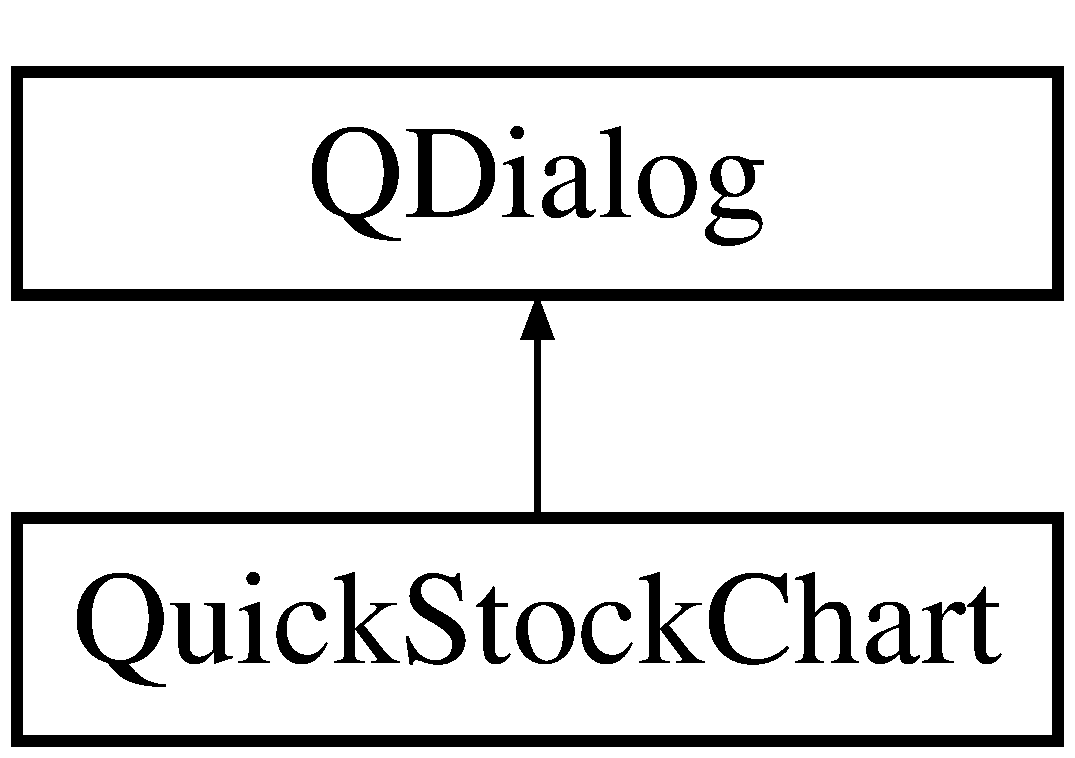
\includegraphics[height=2.000000cm]{class_quick_stock_chart}
\end{center}
\end{figure}
\subsection*{Public Member Functions}
\begin{DoxyCompactItemize}
\item 
\hypertarget{class_quick_stock_chart_abbde5e3fbc236b66dad067b652c58837}{{\bfseries Quick\+Stock\+Chart} (Q\+Widget $\ast$parent=0, Q\+Url Quick\+Stock\+Chart\+Url=Q\+Url(\char`\"{}http\+://www.\+finviz.\+com/chart.\+ashx?t=S\+P\+Y\&ty=c\&ta=1\&p=d\&s=l\char`\"{}))}\label{class_quick_stock_chart_abbde5e3fbc236b66dad067b652c58837}

\end{DoxyCompactItemize}
\subsection*{Private Slots}
\begin{DoxyCompactItemize}
\item 
\hypertarget{class_quick_stock_chart_af99b1a624e729e2328350f38968aa1e1}{void {\bfseries save\+Position} ()}\label{class_quick_stock_chart_af99b1a624e729e2328350f38968aa1e1}

\item 
\hypertarget{class_quick_stock_chart_ac9e5329aad2b5bce87fa46d05da331ef}{void {\bfseries load\+Position} ()}\label{class_quick_stock_chart_ac9e5329aad2b5bce87fa46d05da331ef}

\item 
\hypertarget{class_quick_stock_chart_a764cae6c7bcd52ee0d7fe42dd4b33929}{void {\bfseries close\+Event} (Q\+Close\+Event $\ast$event)}\label{class_quick_stock_chart_a764cae6c7bcd52ee0d7fe42dd4b33929}

\end{DoxyCompactItemize}
\subsection*{Private Attributes}
\begin{DoxyCompactItemize}
\item 
\hypertarget{class_quick_stock_chart_aff762155d7d6c38f87c0fd0ff6733842}{Ui\+::\+Quick\+Stock\+Chart $\ast$ {\bfseries ui}}\label{class_quick_stock_chart_aff762155d7d6c38f87c0fd0ff6733842}

\end{DoxyCompactItemize}


The documentation for this class was generated from the following files\+:\begin{DoxyCompactItemize}
\item 
C\+:/\+Users/\+Q/\+Documents/\+Git\+Hub/\+T\+K\+R\+T\+A\+P/\hyperlink{quickstockchart_8h}{quickstockchart.\+h}\item 
C\+:/\+Users/\+Q/\+Documents/\+Git\+Hub/\+T\+K\+R\+T\+A\+P/\hyperlink{quickstockchart_8cpp}{quickstockchart.\+cpp}\end{DoxyCompactItemize}

\hypertarget{class_rss_client}{\section{Rss\+Client Class Reference}
\label{class_rss_client}\index{Rss\+Client@{Rss\+Client}}
}


The \hyperlink{class_rss_client}{Rss\+Client} class handles the reception and sorting (by date) of multiple R\+S\+S news feeds.  




{\ttfamily \#include $<$rssclient.\+h$>$}

Inheritance diagram for Rss\+Client\+:\begin{figure}[H]
\begin{center}
\leavevmode
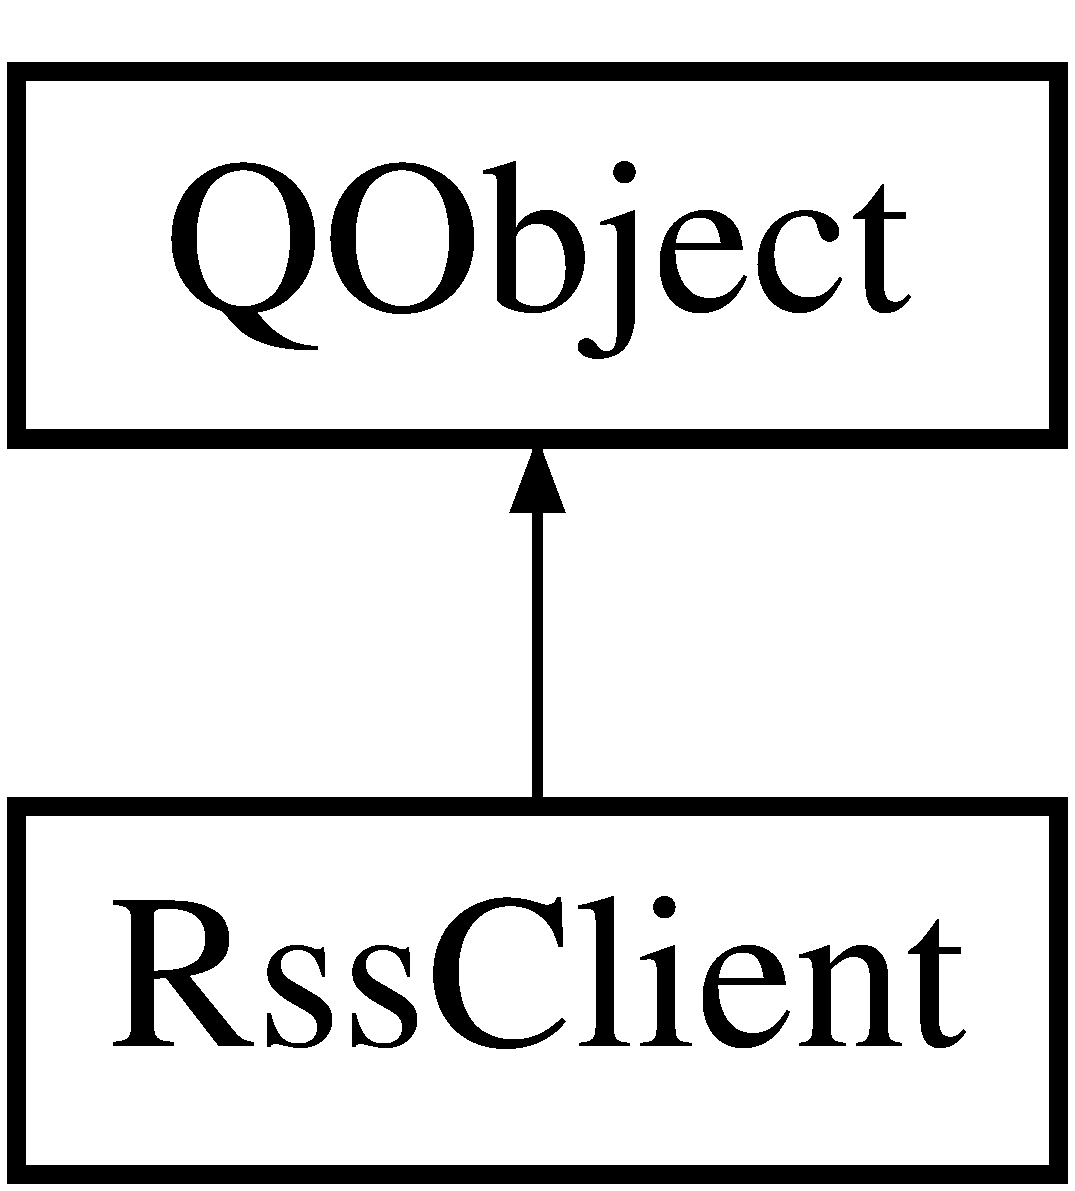
\includegraphics[height=2.000000cm]{class_rss_client}
\end{center}
\end{figure}
\subsection*{Public Slots}
\begin{DoxyCompactItemize}
\item 
\hypertarget{class_rss_client_a2f5ee7ba4e8780c9ed0601b5dd2e6beb}{void \hyperlink{class_rss_client_a2f5ee7ba4e8780c9ed0601b5dd2e6beb}{fetch} ()}\label{class_rss_client_a2f5ee7ba4e8780c9ed0601b5dd2e6beb}

\begin{DoxyCompactList}\small\item\em fetches the first R\+S\+S link. If there are no R\+S\+S links loaded, will do nothing \end{DoxyCompactList}\end{DoxyCompactItemize}
\subsection*{Signals}
\begin{DoxyCompactItemize}
\item 
void \hyperlink{class_rss_client_ab6d60bfd93285070055f5abddc4e3804}{rss\+Finished} (Q\+String\+List title\+\_\+rss, Q\+String\+List link\+\_\+rss, Q\+String\+List date\+\_\+rss)
\begin{DoxyCompactList}\small\item\em Signal used when the R\+S\+S are finished reading. \end{DoxyCompactList}\end{DoxyCompactItemize}
\subsection*{Public Member Functions}
\begin{DoxyCompactItemize}
\item 
\hypertarget{class_rss_client_a99adb986f95f2c8b1b9201d45f4822b1}{\hyperlink{class_rss_client_a99adb986f95f2c8b1b9201d45f4822b1}{Rss\+Client} ()}\label{class_rss_client_a99adb986f95f2c8b1b9201d45f4822b1}

\begin{DoxyCompactList}\small\item\em Constructor. \end{DoxyCompactList}\item 
void \hyperlink{class_rss_client_ac47a9d917d4c52b1e90fe59b6156fa47}{load\+R\+S\+S} (Q\+String\+List list\+\_\+\+R\+S\+S)
\begin{DoxyCompactList}\small\item\em Sets the R\+S\+S links. \end{DoxyCompactList}\end{DoxyCompactItemize}
\subsection*{Private Slots}
\begin{DoxyCompactItemize}
\item 
\hypertarget{class_rss_client_a6ef58c1b978fff1e437d07916b9d5ffb}{void \hyperlink{class_rss_client_a6ef58c1b978fff1e437d07916b9d5ffb}{parse\+Xml} ()}\label{class_rss_client_a6ef58c1b978fff1e437d07916b9d5ffb}

\begin{DoxyCompactList}\small\item\em Parses the X\+M\+L object and extracts the title, date and link information. These are strored in \hyperlink{class_rss_client_ab7a26f3940ef8106cb3cfd81f2e37635}{Rss\+Client\+::\+\_\+model\+\_\+data}. \end{DoxyCompactList}\item 
\hypertarget{class_rss_client_a280dfdaa7e4c1be4cf804c9c8f6f0cd4}{void \hyperlink{class_rss_client_a280dfdaa7e4c1be4cf804c9c8f6f0cd4}{more\+R\+S\+S} ()}\label{class_rss_client_a280dfdaa7e4c1be4cf804c9c8f6f0cd4}

\begin{DoxyCompactList}\small\item\em Fetches every R\+S\+S link after the first and emits the \hyperlink{class_rss_client_ab6d60bfd93285070055f5abddc4e3804}{rss\+Finished} when all the R\+S\+S links are finished reading. \end{DoxyCompactList}\item 
\hypertarget{class_rss_client_a6173e6e7b14eb6a7116e7341ea255015}{void \hyperlink{class_rss_client_a6173e6e7b14eb6a7116e7341ea255015}{ready\+Read} ()}\label{class_rss_client_a6173e6e7b14eb6a7116e7341ea255015}

\begin{DoxyCompactList}\small\item\em Adds the received data to the X\+M\+L object. \end{DoxyCompactList}\item 
\hypertarget{class_rss_client_a91d08eb4371ad934aee0a97d0701bc0b}{void \hyperlink{class_rss_client_a91d08eb4371ad934aee0a97d0701bc0b}{error} (Q\+Network\+Reply\+::\+Network\+Error)}\label{class_rss_client_a91d08eb4371ad934aee0a97d0701bc0b}

\begin{DoxyCompactList}\small\item\em Error handling. \end{DoxyCompactList}\item 
\hypertarget{class_rss_client_a9bd0db5161f3e7b64a9585ea56a0b235}{void \hyperlink{class_rss_client_a9bd0db5161f3e7b64a9585ea56a0b235}{meta\+Data\+Changed} ()}\label{class_rss_client_a9bd0db5161f3e7b64a9585ea56a0b235}

\begin{DoxyCompactList}\small\item\em Used when meta data is changed. \end{DoxyCompactList}\item 
void \hyperlink{class_rss_client_a4133d7464dc3ed28bca7b0537d890e58}{get} (Q\+Url url)
\begin{DoxyCompactList}\small\item\em Sets up the Q\+Network\+Access\+Manager and connects its signals to various slots. \end{DoxyCompactList}\end{DoxyCompactItemize}
\subsection*{Private Member Functions}
\begin{DoxyCompactItemize}
\item 
Q\+Date\+Time \hyperlink{class_rss_client_ad9154be13d0578b3863ad12b1472e72e}{parse\+Date} (Q\+String str\+\_\+date)
\begin{DoxyCompactList}\small\item\em Parses the date and time contained in a Q\+String. This function relies on the \href{http://www.partow.net/programming/datetime/index.html}{\tt Date And Time Parsing Utilities Library} by Arash Partow. \end{DoxyCompactList}\end{DoxyCompactItemize}
\subsection*{Private Attributes}
\begin{DoxyCompactItemize}
\item 
\hypertarget{class_rss_client_ab7a26f3940ef8106cb3cfd81f2e37635}{Q\+Standard\+Item\+Model $\ast$ \hyperlink{class_rss_client_ab7a26f3940ef8106cb3cfd81f2e37635}{\+\_\+model\+\_\+data}}\label{class_rss_client_ab7a26f3940ef8106cb3cfd81f2e37635}

\begin{DoxyCompactList}\small\item\em Contains all the extracted info from the R\+S\+S feeds. \end{DoxyCompactList}\item 
\hypertarget{class_rss_client_a1a302e544e60a4c6d87b780baf5aa44b}{int \hyperlink{class_rss_client_a1a302e544e60a4c6d87b780baf5aa44b}{\+\_\+no\+\_\+data}}\label{class_rss_client_a1a302e544e60a4c6d87b780baf5aa44b}

\begin{DoxyCompactList}\small\item\em Current count of received R\+S\+S news items. \end{DoxyCompactList}\item 
\hypertarget{class_rss_client_ae6ae07ab3ed73a6a58ec4d7aad37fa74}{int \hyperlink{class_rss_client_ae6ae07ab3ed73a6a58ec4d7aad37fa74}{\+\_\+no\+\_\+rss}}\label{class_rss_client_ae6ae07ab3ed73a6a58ec4d7aad37fa74}

\begin{DoxyCompactList}\small\item\em Current count of R\+S\+S feeds. \end{DoxyCompactList}\item 
\hypertarget{class_rss_client_a22dedd159a3374efc3bed38a296b98cc}{Q\+Xml\+Stream\+Reader \hyperlink{class_rss_client_a22dedd159a3374efc3bed38a296b98cc}{\+\_\+xml}}\label{class_rss_client_a22dedd159a3374efc3bed38a296b98cc}

\begin{DoxyCompactList}\small\item\em X\+M\+L object. \end{DoxyCompactList}\item 
\hypertarget{class_rss_client_abdb6d0e6dd2b395548a4a7305a7e1d7d}{Q\+String \hyperlink{class_rss_client_abdb6d0e6dd2b395548a4a7305a7e1d7d}{\+\_\+current\+\_\+tag}}\label{class_rss_client_abdb6d0e6dd2b395548a4a7305a7e1d7d}

\begin{DoxyCompactList}\small\item\em String containing the currently read tag from the X\+M\+L/\+R\+S\+S feed. \end{DoxyCompactList}\item 
\hypertarget{class_rss_client_ac9ec3cd22441d8e597702e73c7a67339}{Q\+String \hyperlink{class_rss_client_ac9ec3cd22441d8e597702e73c7a67339}{\+\_\+date\+\_\+string}}\label{class_rss_client_ac9ec3cd22441d8e597702e73c7a67339}

\begin{DoxyCompactList}\small\item\em String containing the current date from the R\+S\+S News item. \end{DoxyCompactList}\item 
\hypertarget{class_rss_client_a13193830f4d917c6f891a3e75433e72b}{Q\+String \hyperlink{class_rss_client_a13193830f4d917c6f891a3e75433e72b}{\+\_\+link\+\_\+string}}\label{class_rss_client_a13193830f4d917c6f891a3e75433e72b}

\begin{DoxyCompactList}\small\item\em String containing the current link from the R\+S\+S News item. \end{DoxyCompactList}\item 
\hypertarget{class_rss_client_a3ad6f30274197c57d29bbd884b28420d}{Q\+String \hyperlink{class_rss_client_a3ad6f30274197c57d29bbd884b28420d}{\+\_\+title\+\_\+string}}\label{class_rss_client_a3ad6f30274197c57d29bbd884b28420d}

\begin{DoxyCompactList}\small\item\em String containing the current title from the R\+S\+S News item. \end{DoxyCompactList}\item 
\hypertarget{class_rss_client_a2ea54b1553fd8eaa6bb04e2ef829f6eb}{Q\+String\+List \hyperlink{class_rss_client_a2ea54b1553fd8eaa6bb04e2ef829f6eb}{\+\_\+link\+\_\+string\+\_\+list}}\label{class_rss_client_a2ea54b1553fd8eaa6bb04e2ef829f6eb}

\begin{DoxyCompactList}\small\item\em List of stings containing all the U\+R\+Ls for the R\+S\+S feeds to be read. \end{DoxyCompactList}\item 
\hypertarget{class_rss_client_ac97d045a18b36d5c00b44180111ae6bb}{Q\+Network\+Access\+Manager \hyperlink{class_rss_client_ac97d045a18b36d5c00b44180111ae6bb}{\+\_\+manager}}\label{class_rss_client_ac97d045a18b36d5c00b44180111ae6bb}

\begin{DoxyCompactList}\small\item\em The manager used to perform the network request. \end{DoxyCompactList}\item 
\hypertarget{class_rss_client_a1f4d94d00fc34becd2e0f456082a0c45}{Q\+Network\+Reply $\ast$ \hyperlink{class_rss_client_a1f4d94d00fc34becd2e0f456082a0c45}{\+\_\+current\+\_\+reply}}\label{class_rss_client_a1f4d94d00fc34becd2e0f456082a0c45}

\begin{DoxyCompactList}\small\item\em The current network reply. \end{DoxyCompactList}\end{DoxyCompactItemize}


\subsection{Detailed Description}
The \hyperlink{class_rss_client}{Rss\+Client} class handles the reception and sorting (by date) of multiple R\+S\+S news feeds. 

\subsection{Member Function Documentation}
\hypertarget{class_rss_client_a4133d7464dc3ed28bca7b0537d890e58}{\index{Rss\+Client@{Rss\+Client}!get@{get}}
\index{get@{get}!Rss\+Client@{Rss\+Client}}
\subsubsection[{get}]{\setlength{\rightskip}{0pt plus 5cm}void Rss\+Client\+::get (
\begin{DoxyParamCaption}
\item[{Q\+Url}]{url}
\end{DoxyParamCaption}
)\hspace{0.3cm}{\ttfamily [private]}, {\ttfamily [slot]}}}\label{class_rss_client_a4133d7464dc3ed28bca7b0537d890e58}


Sets up the Q\+Network\+Access\+Manager and connects its signals to various slots. 


\begin{DoxyParams}{Parameters}
{\em url} & The url of the R\+S\+S feed to read \\
\hline
\end{DoxyParams}
\hypertarget{class_rss_client_ac47a9d917d4c52b1e90fe59b6156fa47}{\index{Rss\+Client@{Rss\+Client}!load\+R\+S\+S@{load\+R\+S\+S}}
\index{load\+R\+S\+S@{load\+R\+S\+S}!Rss\+Client@{Rss\+Client}}
\subsubsection[{load\+R\+S\+S}]{\setlength{\rightskip}{0pt plus 5cm}void Rss\+Client\+::load\+R\+S\+S (
\begin{DoxyParamCaption}
\item[{Q\+String\+List}]{list\+\_\+\+R\+S\+S}
\end{DoxyParamCaption}
)}}\label{class_rss_client_ac47a9d917d4c52b1e90fe59b6156fa47}


Sets the R\+S\+S links. 


\begin{DoxyParams}{Parameters}
{\em list\+\_\+\+R\+S\+S} & The list of R\+S\+S links \\
\hline
\end{DoxyParams}
\hypertarget{class_rss_client_ad9154be13d0578b3863ad12b1472e72e}{\index{Rss\+Client@{Rss\+Client}!parse\+Date@{parse\+Date}}
\index{parse\+Date@{parse\+Date}!Rss\+Client@{Rss\+Client}}
\subsubsection[{parse\+Date}]{\setlength{\rightskip}{0pt plus 5cm}Q\+Date\+Time Rss\+Client\+::parse\+Date (
\begin{DoxyParamCaption}
\item[{Q\+String}]{str\+\_\+date}
\end{DoxyParamCaption}
)\hspace{0.3cm}{\ttfamily [private]}}}\label{class_rss_client_ad9154be13d0578b3863ad12b1472e72e}


Parses the date and time contained in a Q\+String. This function relies on the \href{http://www.partow.net/programming/datetime/index.html}{\tt Date And Time Parsing Utilities Library} by Arash Partow. 


\begin{DoxyParams}{Parameters}
{\em str\+\_\+date} & The Q\+String containing the date to parse \\
\hline
\end{DoxyParams}
\begin{DoxyReturn}{Returns}
A Q\+Date\+Time containing the parsed date 
\end{DoxyReturn}
\hypertarget{class_rss_client_ab6d60bfd93285070055f5abddc4e3804}{\index{Rss\+Client@{Rss\+Client}!rss\+Finished@{rss\+Finished}}
\index{rss\+Finished@{rss\+Finished}!Rss\+Client@{Rss\+Client}}
\subsubsection[{rss\+Finished}]{\setlength{\rightskip}{0pt plus 5cm}void Rss\+Client\+::rss\+Finished (
\begin{DoxyParamCaption}
\item[{Q\+String\+List}]{title\+\_\+rss, }
\item[{Q\+String\+List}]{link\+\_\+rss, }
\item[{Q\+String\+List}]{date\+\_\+rss}
\end{DoxyParamCaption}
)\hspace{0.3cm}{\ttfamily [signal]}}}\label{class_rss_client_ab6d60bfd93285070055f5abddc4e3804}


Signal used when the R\+S\+S are finished reading. 


\begin{DoxyParams}{Parameters}
{\em title\+\_\+rss} & List of R\+S\+S titles \\
\hline
{\em link\+\_\+rss} & List of the R\+S\+S links \\
\hline
{\em date\+\_\+rss} & List of the R\+S\+S published times \\
\hline
\end{DoxyParams}


The documentation for this class was generated from the following files\+:\begin{DoxyCompactItemize}
\item 
C\+:/\+Users/\+Q/\+Documents/\+Git\+Hub/\+T\+K\+R\+T\+A\+P/\hyperlink{rssclient_8h}{rssclient.\+h}\item 
C\+:/\+Users/\+Q/\+Documents/\+Git\+Hub/\+T\+K\+R\+T\+A\+P/\hyperlink{rssclient_8cpp}{rssclient.\+cpp}\end{DoxyCompactItemize}

\hypertarget{class_t_k_r_t_a_p}{\section{T\+K\+R\+T\+A\+P Class Reference}
\label{class_t_k_r_t_a_p}\index{T\+K\+R\+T\+A\+P@{T\+K\+R\+T\+A\+P}}
}


The main U\+I class.  




{\ttfamily \#include $<$tkrtap.\+h$>$}

Inheritance diagram for T\+K\+R\+T\+A\+P\+:\begin{figure}[H]
\begin{center}
\leavevmode
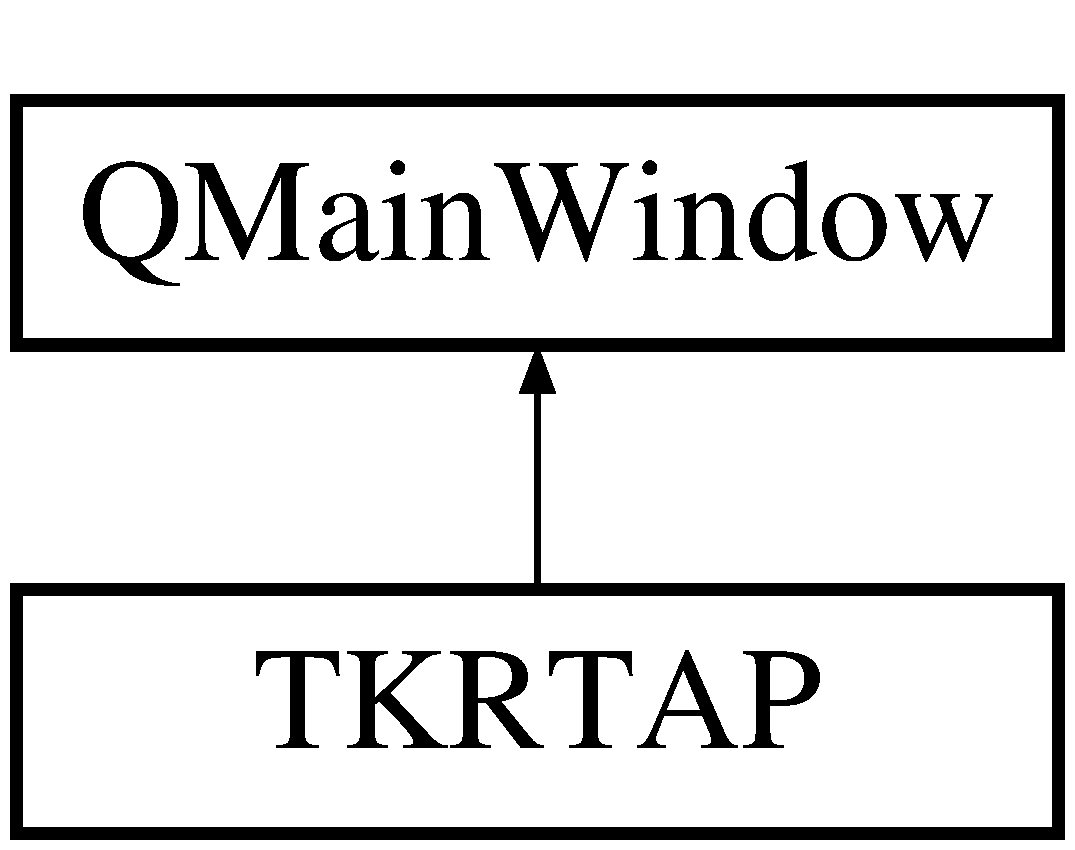
\includegraphics[height=2.000000cm]{class_t_k_r_t_a_p}
\end{center}
\end{figure}
\subsection*{Public Member Functions}
\begin{DoxyCompactItemize}
\item 
\hyperlink{class_t_k_r_t_a_p_ae3eb36f7ee1ed36edc17ac850a6e415a}{T\+K\+R\+T\+A\+P} (Q\+Widget $\ast$parent=0)
\begin{DoxyCompactList}\small\item\em The constructor. \end{DoxyCompactList}\end{DoxyCompactItemize}
\subsection*{Private Slots}
\begin{DoxyCompactItemize}
\item 
void \hyperlink{class_t_k_r_t_a_p_a0fd918db6da7ef497b167f3af9a21204}{link\+S\+E\+C} ()
\begin{DoxyCompactList}\small\item\em Function that opens in a default browser seclive.\+com Link. \end{DoxyCompactList}\item 
void \hyperlink{class_t_k_r_t_a_p_a5f1ebaf5fe11868b7aa882f2c734e4b2}{link\+Charts} ()
\begin{DoxyCompactList}\small\item\em Function that opens in a default browser freestockcharts.\+com Link. \end{DoxyCompactList}\item 
void \hyperlink{class_t_k_r_t_a_p_acefe694e3e0bf827a51817eaaca3e0da}{link\+Screener} ()
\begin{DoxyCompactList}\small\item\em Function that opens in a default browser Finviz Screener Link. \end{DoxyCompactList}\item 
void \hyperlink{class_t_k_r_t_a_p_aeb83e283359840bee97909a92564e324}{link\+Econ} ()
\begin{DoxyCompactList}\small\item\em Function that opens in a default browser tradingeconomics.\+com Link. \end{DoxyCompactList}\item 
void \hyperlink{class_t_k_r_t_a_p_aa0d9e2c05ad6640909eca54f995b04e7}{link\+Fin\+Stat} ()
\begin{DoxyCompactList}\small\item\em Function that opens in a default browser Morningstar financial statements Link. \end{DoxyCompactList}\item 
void \hyperlink{class_t_k_r_t_a_p_a74b55a81eb15e9eee97e901598be20eb}{link\+Analysis} ()
\begin{DoxyCompactList}\small\item\em Function that opens in a default browser Seeking Alpha Link. \end{DoxyCompactList}\item 
void \hyperlink{class_t_k_r_t_a_p_a118fbdc56d14b61c21ee360fb178b393}{link\+Other} ()
\begin{DoxyCompactList}\small\item\em Function that opens in a default browser Google Spreadsheet Link. \end{DoxyCompactList}\item 
\hypertarget{class_t_k_r_t_a_p_a5019b726b6b221933abc42259996a999}{void \hyperlink{class_t_k_r_t_a_p_a5019b726b6b221933abc42259996a999}{on\+\_\+\+Spreadsheet\+\_\+clicked} ()}\label{class_t_k_r_t_a_p_a5019b726b6b221933abc42259996a999}

\begin{DoxyCompactList}\small\item\em Open the link in the default browser of the user. \end{DoxyCompactList}\item 
void \hyperlink{class_t_k_r_t_a_p_a55ad82b64ab31eba3e8ac1aa56e3645e}{on\+\_\+\+Add\+Button\+\_\+clicked} ()
\begin{DoxyCompactList}\small\item\em Adds a stock. \end{DoxyCompactList}\item 
void \hyperlink{class_t_k_r_t_a_p_a56fe0e3c4f6ba41aa41ee94464a7c6c0}{on\+\_\+\+Del\+Button\+\_\+clicked} ()
\begin{DoxyCompactList}\small\item\em Function that deletes a stock. \end{DoxyCompactList}\item 
void \hyperlink{class_t_k_r_t_a_p_a091ace4c0a198698e146d5e4186adb88}{on\+\_\+\+Save\+Button\+\_\+clicked} ()
\begin{DoxyCompactList}\small\item\em Triggers the Save\+Settings Function. \end{DoxyCompactList}\item 
void \hyperlink{class_t_k_r_t_a_p_a3f0d2df000debf0e3d762cd42309ddd1}{Save\+Settings} ()
\begin{DoxyCompactList}\small\item\em Opens the save file dialog. \end{DoxyCompactList}\item 
void \hyperlink{class_t_k_r_t_a_p_a2c5ded6487aad0d51e3c023d597b6072}{on\+\_\+\+Load\+Button\+\_\+clicked} ()
\begin{DoxyCompactList}\small\item\em Triggers the Load\+Settings function when clicked. \end{DoxyCompactList}\item 
void \hyperlink{class_t_k_r_t_a_p_a15cd045fcc12644e07291ef00c9bc6f5}{Load\+Settings} ()
\begin{DoxyCompactList}\small\item\em Opens the load file dialog. \end{DoxyCompactList}\item 
void \hyperlink{class_t_k_r_t_a_p_a5978ee276d97cfbdac62aa6a825d4449}{Load\+Market\+Map} ()
\begin{DoxyCompactList}\small\item\em Opens the Market Map dialog box. \end{DoxyCompactList}\item 
void \hyperlink{class_t_k_r_t_a_p_ac34089a7673199ae27b6cbc3e4f20ffe}{on\+\_\+\+All\+Button\+\_\+clicked} ()
\begin{DoxyCompactList}\small\item\em Triggers all the buttons. \end{DoxyCompactList}\item 
void \hyperlink{class_t_k_r_t_a_p_aea76795d49f0ce78a0f1ddf1bd47cd75}{on\+\_\+\+Spreadsheet\+Button\+Text\+Edit\+\_\+text\+Changed} (const Q\+String \&arg1)
\begin{DoxyCompactList}\small\item\em Function that opens in a default browser the S\+E\+C Link. \end{DoxyCompactList}\item 
void \hyperlink{class_t_k_r_t_a_p_aa01ac37701db845187a9462e703d089f}{on\+\_\+\+Markmap\+Button\+Text\+Edit\+\_\+text\+Changed} (const Q\+String \&arg1)
\begin{DoxyCompactList}\small\item\em Changes the text on the market map button. \end{DoxyCompactList}\item 
void \hyperlink{class_t_k_r_t_a_p_a52aeb4ceba84acce2a98e8e059eeed9f}{on\+\_\+\+Analysis\+Button\+Text\+Edit\+\_\+text\+Changed} (const Q\+String \&arg1)
\begin{DoxyCompactList}\small\item\em Changes the text on the Analysis button. \end{DoxyCompactList}\item 
void \hyperlink{class_t_k_r_t_a_p_a13ba09fe615e6ea1a8aede0589b79bce}{on\+\_\+\+S\+E\+C\+Button\+Text\+Edit\+\_\+text\+Changed} (const Q\+String \&arg1)
\begin{DoxyCompactList}\small\item\em Changes the text on the S\+E\+C button. \end{DoxyCompactList}\item 
void \hyperlink{class_t_k_r_t_a_p_ab614bb00b5d68ea8ddb0c87a028c9687}{on\+\_\+\+Fin\+Stat\+Button\+Text\+Edit\+\_\+text\+Changed} (const Q\+String \&arg1)
\begin{DoxyCompactList}\small\item\em Changes the text on the Financial Statement button. \end{DoxyCompactList}\item 
void \hyperlink{class_t_k_r_t_a_p_a13c4a949a02a82b73639292611392f03}{on\+\_\+\+Econ\+Button\+Text\+Edit\+\_\+text\+Changed} (const Q\+String \&arg1)
\begin{DoxyCompactList}\small\item\em Changes the text on the Economic indicators button. \end{DoxyCompactList}\item 
void \hyperlink{class_t_k_r_t_a_p_a496a9cdf9ca2b12fef3201e2ccb8eac5}{on\+\_\+\+Screener\+Button\+Text\+Edit\+\_\+text\+Changed} (const Q\+String \&arg1)
\begin{DoxyCompactList}\small\item\em Changes the text on the Screener button. \end{DoxyCompactList}\item 
void \hyperlink{class_t_k_r_t_a_p_a05b206d46bedfd8063e85f4fbc331b11}{on\+\_\+\+Charts\+Button\+Text\+Edit\+\_\+text\+Changed} (const Q\+String \&arg1)
\begin{DoxyCompactList}\small\item\em Changes the text on the Charts button. \end{DoxyCompactList}\item 
\hypertarget{class_t_k_r_t_a_p_a9eb892a2a12c96d79d95968942811269}{void \hyperlink{class_t_k_r_t_a_p_a9eb892a2a12c96d79d95968942811269}{set\+Scroll\+Speed} ()}\label{class_t_k_r_t_a_p_a9eb892a2a12c96d79d95968942811269}

\begin{DoxyCompactList}\small\item\em Changes the speed of the L\+E\+D Panel. \end{DoxyCompactList}\item 
void \hyperlink{class_t_k_r_t_a_p_a6ddb840aa530eb4834f137907c82309f}{set\+Couleurs} ()
\begin{DoxyCompactList}\small\item\em Changes the colors of the L\+E\+D Panel. \end{DoxyCompactList}\item 
void \hyperlink{class_t_k_r_t_a_p_ad7900d7be69bfb772b4aa3de070dcb98}{set\+Ligne1} ()
\begin{DoxyCompactList}\small\item\em Changes the text on the first line of the L\+E\+D Panel. \end{DoxyCompactList}\item 
void \hyperlink{class_t_k_r_t_a_p_a2a86e3fb126a976efa13aae2bbf3d231}{set\+Ligne2} ()
\begin{DoxyCompactList}\small\item\em Changes the text on the second line of the L\+E\+D Panel. \end{DoxyCompactList}\item 
\hypertarget{class_t_k_r_t_a_p_ad037f38e28ef942688d7ad6e0bf4a62c}{void \hyperlink{class_t_k_r_t_a_p_ad037f38e28ef942688d7ad6e0bf4a62c}{toggle\+Serial\+Port} ()}\label{class_t_k_r_t_a_p_ad037f38e28ef942688d7ad6e0bf4a62c}

\begin{DoxyCompactList}\small\item\em Activates the necessary functions to start outputing data to the L\+E\+D panel. \end{DoxyCompactList}\item 
void \hyperlink{class_t_k_r_t_a_p_a7e405d4c3d7f022889242376072ce821}{Removing\+\_\+\+Duplicates\+\_\+\+R\+S\+S} ()
\begin{DoxyCompactList}\small\item\em Functions that removes any duplicates in the R\+S\+S link list. \end{DoxyCompactList}\item 
void \hyperlink{class_t_k_r_t_a_p_a54b652ca1f240769140b278e0e4a4ddb}{on\+\_\+list\+View\+\_\+double\+Clicked} (const Q\+Model\+Index \&index)
\begin{DoxyCompactList}\small\item\em Triggers the quick stock chart dialog of the stock clicked. \end{DoxyCompactList}\item 
\hypertarget{class_t_k_r_t_a_p_a0d824d019f7724b276db0622bd43adbf}{void \hyperlink{class_t_k_r_t_a_p_a0d824d019f7724b276db0622bd43adbf}{open\+Stock\+Chart} (Q\+String ticker)}\label{class_t_k_r_t_a_p_a0d824d019f7724b276db0622bd43adbf}

\begin{DoxyCompactList}\small\item\em Opens the Finviz stock chart of the inputed ticker. \end{DoxyCompactList}\item 
Q\+String\+List \hyperlink{class_t_k_r_t_a_p_aa8df0b689d8e9c9ca53e040e55ae96c4}{Generate\+Stock\+R\+S\+S} ()
\begin{DoxyCompactList}\small\item\em Creates R\+S\+S links for each stocks. \end{DoxyCompactList}\item 
void \hyperlink{class_t_k_r_t_a_p_a3d229ca32c81efcd046e2cc73c29455a}{on\+\_\+button\+\_\+add\+\_\+link\+\_\+clicked} ()
\begin{DoxyCompactList}\small\item\em Adds a editable line to the R\+S\+S link list. \end{DoxyCompactList}\item 
void \hyperlink{class_t_k_r_t_a_p_a9d26be9315aafb9afc2a134ea9d1ed0b}{on\+\_\+button\+\_\+remove\+\_\+link\+\_\+clicked} ()
\begin{DoxyCompactList}\small\item\em Deletes the selected link. \end{DoxyCompactList}\item 
void \hyperlink{class_t_k_r_t_a_p_ad764cc0d854eb1cf61ad741de1b78368}{on\+\_\+\+Add\+Stock\+R\+S\+S\+Button\+\_\+clicked} ()
\begin{DoxyCompactList}\small\item\em Adds a R\+S\+S link for each stock in watchlist. \end{DoxyCompactList}\item 
void \hyperlink{class_t_k_r_t_a_p_a67ebb1c57c2e2a05a7750e0e42d1b500}{on\+\_\+button\+\_\+clear\+\_\+\+R\+S\+S\+\_\+links\+\_\+clicked} ()
\begin{DoxyCompactList}\small\item\em Clears the R\+S\+S link list. \end{DoxyCompactList}\item 
void \hyperlink{class_t_k_r_t_a_p_adb0ea6e18fbf661f2bf52655f552b907}{timer\+Start} ()
\begin{DoxyCompactList}\small\item\em Starts the timer. \end{DoxyCompactList}\item 
void \hyperlink{class_t_k_r_t_a_p_a6bdc036a4c99e281cc12fb7ab81e8922}{timer\+End} ()
\begin{DoxyCompactList}\small\item\em Ends the timer. \end{DoxyCompactList}\item 
void \hyperlink{class_t_k_r_t_a_p_a9742278d8b60423159e21585bbe1c68b}{on\+\_\+\+Auth\+Tokenpush\+Button\+\_\+clicked} ()
\begin{DoxyCompactList}\small\item\em Link to the Quandl Auth Token web page. \end{DoxyCompactList}\item 
void \hyperlink{class_t_k_r_t_a_p_ad012d6c7aad3cfcc06f5df8a392d308b}{validate\+\_\+tickers} ()
\begin{DoxyCompactList}\small\item\em Check if the user input is valid and if not deletes it. \end{DoxyCompactList}\item 
void \hyperlink{class_t_k_r_t_a_p_a0dc4e02bce5f50d8616a7118a021be34}{J\+S\+O\+N\+Parse\+Complete} (Q\+String\+List txt\+\_\+list, Q\+String colour\+\_\+text)
\begin{DoxyCompactList}\small\item\em Formats the stock quotes results. \end{DoxyCompactList}\item 
void \hyperlink{class_t_k_r_t_a_p_a9105ea4fbf86ffb8e373275677ea99ee}{Setup\+Request} ()
\begin{DoxyCompactList}\small\item\em Updates the stock quotes. \end{DoxyCompactList}\item 
void \hyperlink{class_t_k_r_t_a_p_a2e63c2e8c0b9f5662b06e8686eac0e64}{start\+R\+S\+S} ()
\begin{DoxyCompactList}\small\item\em Starts the R\+S\+S search. \end{DoxyCompactList}\item 
void \hyperlink{class_t_k_r_t_a_p_adec88a87264a22575064eb9c03eecfc7}{update\+Table} (Q\+String\+List str\+\_\+list, Q\+String\+List link\+\_\+rss, Q\+String\+List time\+\_\+rss)
\begin{DoxyCompactList}\small\item\em Updates the R\+S\+S results list in the U\+I. \end{DoxyCompactList}\item 
void \hyperlink{class_t_k_r_t_a_p_a0dd268ebec54f111eef86da401f459a1}{open\+R\+S\+S\+Link} (Q\+List\+Widget\+Item $\ast$item)
\begin{DoxyCompactList}\small\item\em Opens the linked R\+S\+S. \end{DoxyCompactList}\item 
void \hyperlink{class_t_k_r_t_a_p_afbf6f2c24b041c0834c72d96452638bd}{on\+\_\+\+Save\+\_\+\+Button\+\_\+\+R\+S\+S\+\_\+clicked} ()
\begin{DoxyCompactList}\small\item\em Triggers the save file dialog for the R\+S\+S link list. \end{DoxyCompactList}\item 
void \hyperlink{class_t_k_r_t_a_p_ac99a293ac859f4b8e9f3b539c0fe1889}{on\+\_\+\+Load\+\_\+\+Button\+\_\+\+R\+S\+S\+\_\+clicked} ()
\begin{DoxyCompactList}\small\item\em Triggers the load file dialog for the R\+S\+S link list. \end{DoxyCompactList}\end{DoxyCompactItemize}
\subsection*{Private Attributes}
\begin{DoxyCompactItemize}
\item 
\hypertarget{class_t_k_r_t_a_p_a6bbf119b4d676391d255cccff61fd3db}{\hyperlink{class_json_query}{Json\+Query} $\ast$ \hyperlink{class_t_k_r_t_a_p_a6bbf119b4d676391d255cccff61fd3db}{\+\_\+\+J\+S\+O\+N\+\_\+query}}\label{class_t_k_r_t_a_p_a6bbf119b4d676391d255cccff61fd3db}

\begin{DoxyCompactList}\small\item\em J\+S\+O\+N query object. \end{DoxyCompactList}\item 
\hypertarget{class_t_k_r_t_a_p_aa5c0808ed62d03e2429251f24ce9f1ed}{Ui\+::\+T\+K\+R\+T\+A\+P $\ast$ \hyperlink{class_t_k_r_t_a_p_aa5c0808ed62d03e2429251f24ce9f1ed}{ui}}\label{class_t_k_r_t_a_p_aa5c0808ed62d03e2429251f24ce9f1ed}

\begin{DoxyCompactList}\small\item\em The main U\+I. \end{DoxyCompactList}\item 
\hypertarget{class_t_k_r_t_a_p_ae1b640da392aa1223efadd00e9ab18ef}{Q\+String\+List \hyperlink{class_t_k_r_t_a_p_ae1b640da392aa1223efadd00e9ab18ef}{\+\_\+rss\+\_\+title}}\label{class_t_k_r_t_a_p_ae1b640da392aa1223efadd00e9ab18ef}

\begin{DoxyCompactList}\small\item\em String list containing the R\+S\+S articles titles. \end{DoxyCompactList}\item 
\hypertarget{class_t_k_r_t_a_p_a9ff67f4d9206e5a8b76812497c83680e}{Q\+String\+List \hyperlink{class_t_k_r_t_a_p_a9ff67f4d9206e5a8b76812497c83680e}{\+\_\+rss\+\_\+link}}\label{class_t_k_r_t_a_p_a9ff67f4d9206e5a8b76812497c83680e}

\begin{DoxyCompactList}\small\item\em String list containing the R\+S\+S articles links. \end{DoxyCompactList}\item 
\hypertarget{class_t_k_r_t_a_p_aecca4344eb3c1de07ee5d9269dd288ca}{Q\+String\+List \hyperlink{class_t_k_r_t_a_p_aecca4344eb3c1de07ee5d9269dd288ca}{\+\_\+rss\+\_\+time}}\label{class_t_k_r_t_a_p_aecca4344eb3c1de07ee5d9269dd288ca}

\begin{DoxyCompactList}\small\item\em String list containing the R\+S\+S articles published times. \end{DoxyCompactList}\item 
\hypertarget{class_t_k_r_t_a_p_ac88066b0fa124f52e8755b8d0e034c66}{\hyperlink{class_rss_client}{Rss\+Client} $\ast$ \hyperlink{class_t_k_r_t_a_p_ac88066b0fa124f52e8755b8d0e034c66}{\+\_\+rss\+\_\+client}}\label{class_t_k_r_t_a_p_ac88066b0fa124f52e8755b8d0e034c66}

\begin{DoxyCompactList}\small\item\em Pointer to the R\+S\+S client. \end{DoxyCompactList}\item 
\hypertarget{class_t_k_r_t_a_p_a01c02cbbb5b6939837aaf07ff86c3d99}{Q\+String\+List\+Model $\ast$ \hyperlink{class_t_k_r_t_a_p_a01c02cbbb5b6939837aaf07ff86c3d99}{model}}\label{class_t_k_r_t_a_p_a01c02cbbb5b6939837aaf07ff86c3d99}

\begin{DoxyCompactList}\small\item\em Model containing the tickers. \end{DoxyCompactList}\item 
\hypertarget{class_t_k_r_t_a_p_a8b4b0e92489a64cf5cd8276f77e6da9a}{Q\+String\+List\+Model $\ast$ \hyperlink{class_t_k_r_t_a_p_a8b4b0e92489a64cf5cd8276f77e6da9a}{R\+S\+Slinklistmodel}}\label{class_t_k_r_t_a_p_a8b4b0e92489a64cf5cd8276f77e6da9a}

\begin{DoxyCompactList}\small\item\em Model containing the R\+S\+S links. \end{DoxyCompactList}\item 
\hypertarget{class_t_k_r_t_a_p_aeef7fe3150545933ebe5f6043d2eb765}{\hyperlink{class_market_map_view}{Market\+Map\+View} $\ast$ \hyperlink{class_t_k_r_t_a_p_aeef7fe3150545933ebe5f6043d2eb765}{m\+Dialog}}\label{class_t_k_r_t_a_p_aeef7fe3150545933ebe5f6043d2eb765}

\begin{DoxyCompactList}\small\item\em Dialog box of the Market Map. \end{DoxyCompactList}\item 
\hypertarget{class_t_k_r_t_a_p_abac3af7f25f39fb36ba72118cf210a9c}{\hyperlink{class_quick_stock_chart}{Quick\+Stock\+Chart} $\ast$ \hyperlink{class_t_k_r_t_a_p_abac3af7f25f39fb36ba72118cf210a9c}{m\+Dialog2}}\label{class_t_k_r_t_a_p_abac3af7f25f39fb36ba72118cf210a9c}

\begin{DoxyCompactList}\small\item\em Dialog box of the Quick finviz stock chart. \end{DoxyCompactList}\item 
\hypertarget{class_t_k_r_t_a_p_a5cfe8b9a7354e3b2d2bf13380e1bca10}{\hyperlink{class_matrice_rgb}{Matrice\+Rgb} $\ast$ \hyperlink{class_t_k_r_t_a_p_a5cfe8b9a7354e3b2d2bf13380e1bca10}{\+\_\+matrice}}\label{class_t_k_r_t_a_p_a5cfe8b9a7354e3b2d2bf13380e1bca10}

\begin{DoxyCompactList}\small\item\em Pointer to the matrix. \end{DoxyCompactList}\item 
\hypertarget{class_t_k_r_t_a_p_a70b9df534de6fd98d382d19d2187c081}{Q\+String \hyperlink{class_t_k_r_t_a_p_a70b9df534de6fd98d382d19d2187c081}{\+\_\+nom\+\_\+port}}\label{class_t_k_r_t_a_p_a70b9df534de6fd98d382d19d2187c081}

\begin{DoxyCompactList}\small\item\em The port name used for the matrix. \end{DoxyCompactList}\item 
\hypertarget{class_t_k_r_t_a_p_afac0c2f9700ac220009573a74688f773}{Q\+Timer $\ast$ \hyperlink{class_t_k_r_t_a_p_afac0c2f9700ac220009573a74688f773}{Ticker\+\_\+\+Timer}}\label{class_t_k_r_t_a_p_afac0c2f9700ac220009573a74688f773}

\begin{DoxyCompactList}\small\item\em Timer used to refresh the stock info (prices, etc) \end{DoxyCompactList}\item 
\hypertarget{class_t_k_r_t_a_p_ab1d5dfc208843cd507a348086e862008}{Q\+Timer $\ast$ \hyperlink{class_t_k_r_t_a_p_ab1d5dfc208843cd507a348086e862008}{R\+S\+S\+\_\+\+Timer}}\label{class_t_k_r_t_a_p_ab1d5dfc208843cd507a348086e862008}

\begin{DoxyCompactList}\small\item\em Timer used to refresh the R\+S\+S articles. \end{DoxyCompactList}\end{DoxyCompactItemize}


\subsection{Detailed Description}
The main U\+I class. 

\subsection{Constructor \& Destructor Documentation}
\hypertarget{class_t_k_r_t_a_p_ae3eb36f7ee1ed36edc17ac850a6e415a}{\index{T\+K\+R\+T\+A\+P@{T\+K\+R\+T\+A\+P}!T\+K\+R\+T\+A\+P@{T\+K\+R\+T\+A\+P}}
\index{T\+K\+R\+T\+A\+P@{T\+K\+R\+T\+A\+P}!T\+K\+R\+T\+A\+P@{T\+K\+R\+T\+A\+P}}
\subsubsection[{T\+K\+R\+T\+A\+P}]{\setlength{\rightskip}{0pt plus 5cm}T\+K\+R\+T\+A\+P\+::\+T\+K\+R\+T\+A\+P (
\begin{DoxyParamCaption}
\item[{Q\+Widget $\ast$}]{parent = {\ttfamily 0}}
\end{DoxyParamCaption}
)\hspace{0.3cm}{\ttfamily [explicit]}}}\label{class_t_k_r_t_a_p_ae3eb36f7ee1ed36edc17ac850a6e415a}


The constructor. 


\begin{DoxyParams}{Parameters}
{\em parent} & The parent widget \\
\hline
\end{DoxyParams}


\subsection{Member Function Documentation}
\hypertarget{class_t_k_r_t_a_p_aa8df0b689d8e9c9ca53e040e55ae96c4}{\index{T\+K\+R\+T\+A\+P@{T\+K\+R\+T\+A\+P}!Generate\+Stock\+R\+S\+S@{Generate\+Stock\+R\+S\+S}}
\index{Generate\+Stock\+R\+S\+S@{Generate\+Stock\+R\+S\+S}!T\+K\+R\+T\+A\+P@{T\+K\+R\+T\+A\+P}}
\subsubsection[{Generate\+Stock\+R\+S\+S}]{\setlength{\rightskip}{0pt plus 5cm}Q\+String\+List T\+K\+R\+T\+A\+P\+::\+Generate\+Stock\+R\+S\+S (
\begin{DoxyParamCaption}
{}
\end{DoxyParamCaption}
)\hspace{0.3cm}{\ttfamily [private]}, {\ttfamily [slot]}}}\label{class_t_k_r_t_a_p_aa8df0b689d8e9c9ca53e040e55ae96c4}


Creates R\+S\+S links for each stocks. 

Activates the necessary functions to start outputing data to the L\+E\+D panel.

\begin{DoxyReturn}{Returns}
The full list R\+S\+S url for each stock 
\end{DoxyReturn}
\hypertarget{class_t_k_r_t_a_p_a0dc4e02bce5f50d8616a7118a021be34}{\index{T\+K\+R\+T\+A\+P@{T\+K\+R\+T\+A\+P}!J\+S\+O\+N\+Parse\+Complete@{J\+S\+O\+N\+Parse\+Complete}}
\index{J\+S\+O\+N\+Parse\+Complete@{J\+S\+O\+N\+Parse\+Complete}!T\+K\+R\+T\+A\+P@{T\+K\+R\+T\+A\+P}}
\subsubsection[{J\+S\+O\+N\+Parse\+Complete}]{\setlength{\rightskip}{0pt plus 5cm}void T\+K\+R\+T\+A\+P\+::\+J\+S\+O\+N\+Parse\+Complete (
\begin{DoxyParamCaption}
\item[{Q\+String\+List}]{txt\+\_\+list, }
\item[{Q\+String}]{colour\+\_\+text}
\end{DoxyParamCaption}
)\hspace{0.3cm}{\ttfamily [private]}, {\ttfamily [slot]}}}\label{class_t_k_r_t_a_p_a0dc4e02bce5f50d8616a7118a021be34}


Formats the stock quotes results. 

Passes the formatted String List from to J\+S\+O\+N requests to the different parts of the U\+I.


\begin{DoxyParams}{Parameters}
{\em txt\+\_\+list} & The received String\+List \\
\hline
{\em colour\+\_\+text} & The colour code for the string that will be sent to the R\+G\+B matrix \\
\hline
\end{DoxyParams}
\hypertarget{class_t_k_r_t_a_p_a74b55a81eb15e9eee97e901598be20eb}{\index{T\+K\+R\+T\+A\+P@{T\+K\+R\+T\+A\+P}!link\+Analysis@{link\+Analysis}}
\index{link\+Analysis@{link\+Analysis}!T\+K\+R\+T\+A\+P@{T\+K\+R\+T\+A\+P}}
\subsubsection[{link\+Analysis}]{\setlength{\rightskip}{0pt plus 5cm}void T\+K\+R\+T\+A\+P\+::link\+Analysis (
\begin{DoxyParamCaption}
{}
\end{DoxyParamCaption}
)\hspace{0.3cm}{\ttfamily [private]}, {\ttfamily [slot]}}}\label{class_t_k_r_t_a_p_a74b55a81eb15e9eee97e901598be20eb}


Function that opens in a default browser Seeking Alpha Link. 

Open the link in the default browser of the user. \hypertarget{class_t_k_r_t_a_p_a5f1ebaf5fe11868b7aa882f2c734e4b2}{\index{T\+K\+R\+T\+A\+P@{T\+K\+R\+T\+A\+P}!link\+Charts@{link\+Charts}}
\index{link\+Charts@{link\+Charts}!T\+K\+R\+T\+A\+P@{T\+K\+R\+T\+A\+P}}
\subsubsection[{link\+Charts}]{\setlength{\rightskip}{0pt plus 5cm}void T\+K\+R\+T\+A\+P\+::link\+Charts (
\begin{DoxyParamCaption}
{}
\end{DoxyParamCaption}
)\hspace{0.3cm}{\ttfamily [private]}, {\ttfamily [slot]}}}\label{class_t_k_r_t_a_p_a5f1ebaf5fe11868b7aa882f2c734e4b2}


Function that opens in a default browser freestockcharts.\+com Link. 

Open the link in the default browser of the user. \hypertarget{class_t_k_r_t_a_p_aeb83e283359840bee97909a92564e324}{\index{T\+K\+R\+T\+A\+P@{T\+K\+R\+T\+A\+P}!link\+Econ@{link\+Econ}}
\index{link\+Econ@{link\+Econ}!T\+K\+R\+T\+A\+P@{T\+K\+R\+T\+A\+P}}
\subsubsection[{link\+Econ}]{\setlength{\rightskip}{0pt plus 5cm}void T\+K\+R\+T\+A\+P\+::link\+Econ (
\begin{DoxyParamCaption}
{}
\end{DoxyParamCaption}
)\hspace{0.3cm}{\ttfamily [private]}, {\ttfamily [slot]}}}\label{class_t_k_r_t_a_p_aeb83e283359840bee97909a92564e324}


Function that opens in a default browser tradingeconomics.\+com Link. 

Open the link in the default browser of the user. \hypertarget{class_t_k_r_t_a_p_aa0d9e2c05ad6640909eca54f995b04e7}{\index{T\+K\+R\+T\+A\+P@{T\+K\+R\+T\+A\+P}!link\+Fin\+Stat@{link\+Fin\+Stat}}
\index{link\+Fin\+Stat@{link\+Fin\+Stat}!T\+K\+R\+T\+A\+P@{T\+K\+R\+T\+A\+P}}
\subsubsection[{link\+Fin\+Stat}]{\setlength{\rightskip}{0pt plus 5cm}void T\+K\+R\+T\+A\+P\+::link\+Fin\+Stat (
\begin{DoxyParamCaption}
{}
\end{DoxyParamCaption}
)\hspace{0.3cm}{\ttfamily [private]}, {\ttfamily [slot]}}}\label{class_t_k_r_t_a_p_aa0d9e2c05ad6640909eca54f995b04e7}


Function that opens in a default browser Morningstar financial statements Link. 

Open the link in the default browser of the user. \hypertarget{class_t_k_r_t_a_p_a118fbdc56d14b61c21ee360fb178b393}{\index{T\+K\+R\+T\+A\+P@{T\+K\+R\+T\+A\+P}!link\+Other@{link\+Other}}
\index{link\+Other@{link\+Other}!T\+K\+R\+T\+A\+P@{T\+K\+R\+T\+A\+P}}
\subsubsection[{link\+Other}]{\setlength{\rightskip}{0pt plus 5cm}void T\+K\+R\+T\+A\+P\+::link\+Other (
\begin{DoxyParamCaption}
{}
\end{DoxyParamCaption}
)\hspace{0.3cm}{\ttfamily [private]}, {\ttfamily [slot]}}}\label{class_t_k_r_t_a_p_a118fbdc56d14b61c21ee360fb178b393}


Function that opens in a default browser Google Spreadsheet Link. 

Open the link in the default browser of the user. \hypertarget{class_t_k_r_t_a_p_acefe694e3e0bf827a51817eaaca3e0da}{\index{T\+K\+R\+T\+A\+P@{T\+K\+R\+T\+A\+P}!link\+Screener@{link\+Screener}}
\index{link\+Screener@{link\+Screener}!T\+K\+R\+T\+A\+P@{T\+K\+R\+T\+A\+P}}
\subsubsection[{link\+Screener}]{\setlength{\rightskip}{0pt plus 5cm}void T\+K\+R\+T\+A\+P\+::link\+Screener (
\begin{DoxyParamCaption}
{}
\end{DoxyParamCaption}
)\hspace{0.3cm}{\ttfamily [private]}, {\ttfamily [slot]}}}\label{class_t_k_r_t_a_p_acefe694e3e0bf827a51817eaaca3e0da}


Function that opens in a default browser Finviz Screener Link. 

Open the link in the default browser of the user. \hypertarget{class_t_k_r_t_a_p_a0fd918db6da7ef497b167f3af9a21204}{\index{T\+K\+R\+T\+A\+P@{T\+K\+R\+T\+A\+P}!link\+S\+E\+C@{link\+S\+E\+C}}
\index{link\+S\+E\+C@{link\+S\+E\+C}!T\+K\+R\+T\+A\+P@{T\+K\+R\+T\+A\+P}}
\subsubsection[{link\+S\+E\+C}]{\setlength{\rightskip}{0pt plus 5cm}void T\+K\+R\+T\+A\+P\+::link\+S\+E\+C (
\begin{DoxyParamCaption}
{}
\end{DoxyParamCaption}
)\hspace{0.3cm}{\ttfamily [private]}, {\ttfamily [slot]}}}\label{class_t_k_r_t_a_p_a0fd918db6da7ef497b167f3af9a21204}


Function that opens in a default browser seclive.\+com Link. 

Open the link in the default browser of the user. \hypertarget{class_t_k_r_t_a_p_a5978ee276d97cfbdac62aa6a825d4449}{\index{T\+K\+R\+T\+A\+P@{T\+K\+R\+T\+A\+P}!Load\+Market\+Map@{Load\+Market\+Map}}
\index{Load\+Market\+Map@{Load\+Market\+Map}!T\+K\+R\+T\+A\+P@{T\+K\+R\+T\+A\+P}}
\subsubsection[{Load\+Market\+Map}]{\setlength{\rightskip}{0pt plus 5cm}void T\+K\+R\+T\+A\+P\+::\+Load\+Market\+Map (
\begin{DoxyParamCaption}
{}
\end{DoxyParamCaption}
)\hspace{0.3cm}{\ttfamily [private]}, {\ttfamily [slot]}}}\label{class_t_k_r_t_a_p_a5978ee276d97cfbdac62aa6a825d4449}


Opens the Market Map dialog box. 

Open the link of the Finviz Market\+Map in a browser customized for it. \hypertarget{class_t_k_r_t_a_p_a15cd045fcc12644e07291ef00c9bc6f5}{\index{T\+K\+R\+T\+A\+P@{T\+K\+R\+T\+A\+P}!Load\+Settings@{Load\+Settings}}
\index{Load\+Settings@{Load\+Settings}!T\+K\+R\+T\+A\+P@{T\+K\+R\+T\+A\+P}}
\subsubsection[{Load\+Settings}]{\setlength{\rightskip}{0pt plus 5cm}void T\+K\+R\+T\+A\+P\+::\+Load\+Settings (
\begin{DoxyParamCaption}
{}
\end{DoxyParamCaption}
)\hspace{0.3cm}{\ttfamily [private]}, {\ttfamily [slot]}}}\label{class_t_k_r_t_a_p_a15cd045fcc12644e07291ef00c9bc6f5}


Opens the load file dialog. 

Loads all the user settings. \hypertarget{class_t_k_r_t_a_p_a55ad82b64ab31eba3e8ac1aa56e3645e}{\index{T\+K\+R\+T\+A\+P@{T\+K\+R\+T\+A\+P}!on\+\_\+\+Add\+Button\+\_\+clicked@{on\+\_\+\+Add\+Button\+\_\+clicked}}
\index{on\+\_\+\+Add\+Button\+\_\+clicked@{on\+\_\+\+Add\+Button\+\_\+clicked}!T\+K\+R\+T\+A\+P@{T\+K\+R\+T\+A\+P}}
\subsubsection[{on\+\_\+\+Add\+Button\+\_\+clicked}]{\setlength{\rightskip}{0pt plus 5cm}void T\+K\+R\+T\+A\+P\+::on\+\_\+\+Add\+Button\+\_\+clicked (
\begin{DoxyParamCaption}
{}
\end{DoxyParamCaption}
)\hspace{0.3cm}{\ttfamily [private]}, {\ttfamily [slot]}}}\label{class_t_k_r_t_a_p_a55ad82b64ab31eba3e8ac1aa56e3645e}


Adds a stock. 

Adds a line to the ticker list and enables editing of that line. \hypertarget{class_t_k_r_t_a_p_ad764cc0d854eb1cf61ad741de1b78368}{\index{T\+K\+R\+T\+A\+P@{T\+K\+R\+T\+A\+P}!on\+\_\+\+Add\+Stock\+R\+S\+S\+Button\+\_\+clicked@{on\+\_\+\+Add\+Stock\+R\+S\+S\+Button\+\_\+clicked}}
\index{on\+\_\+\+Add\+Stock\+R\+S\+S\+Button\+\_\+clicked@{on\+\_\+\+Add\+Stock\+R\+S\+S\+Button\+\_\+clicked}!T\+K\+R\+T\+A\+P@{T\+K\+R\+T\+A\+P}}
\subsubsection[{on\+\_\+\+Add\+Stock\+R\+S\+S\+Button\+\_\+clicked}]{\setlength{\rightskip}{0pt plus 5cm}void T\+K\+R\+T\+A\+P\+::on\+\_\+\+Add\+Stock\+R\+S\+S\+Button\+\_\+clicked (
\begin{DoxyParamCaption}
{}
\end{DoxyParamCaption}
)\hspace{0.3cm}{\ttfamily [private]}, {\ttfamily [slot]}}}\label{class_t_k_r_t_a_p_ad764cc0d854eb1cf61ad741de1b78368}


Adds a R\+S\+S link for each stock in watchlist. 

When the button is clicked an R\+S\+S link is created for each stock ticker in the stock ticker list by calling Generate\+Stock\+R\+S\+S. \hypertarget{class_t_k_r_t_a_p_ac34089a7673199ae27b6cbc3e4f20ffe}{\index{T\+K\+R\+T\+A\+P@{T\+K\+R\+T\+A\+P}!on\+\_\+\+All\+Button\+\_\+clicked@{on\+\_\+\+All\+Button\+\_\+clicked}}
\index{on\+\_\+\+All\+Button\+\_\+clicked@{on\+\_\+\+All\+Button\+\_\+clicked}!T\+K\+R\+T\+A\+P@{T\+K\+R\+T\+A\+P}}
\subsubsection[{on\+\_\+\+All\+Button\+\_\+clicked}]{\setlength{\rightskip}{0pt plus 5cm}void T\+K\+R\+T\+A\+P\+::on\+\_\+\+All\+Button\+\_\+clicked (
\begin{DoxyParamCaption}
{}
\end{DoxyParamCaption}
)\hspace{0.3cm}{\ttfamily [private]}, {\ttfamily [slot]}}}\label{class_t_k_r_t_a_p_ac34089a7673199ae27b6cbc3e4f20ffe}


Triggers all the buttons. 

Trigger all the link buttons. \hypertarget{class_t_k_r_t_a_p_a52aeb4ceba84acce2a98e8e059eeed9f}{\index{T\+K\+R\+T\+A\+P@{T\+K\+R\+T\+A\+P}!on\+\_\+\+Analysis\+Button\+Text\+Edit\+\_\+text\+Changed@{on\+\_\+\+Analysis\+Button\+Text\+Edit\+\_\+text\+Changed}}
\index{on\+\_\+\+Analysis\+Button\+Text\+Edit\+\_\+text\+Changed@{on\+\_\+\+Analysis\+Button\+Text\+Edit\+\_\+text\+Changed}!T\+K\+R\+T\+A\+P@{T\+K\+R\+T\+A\+P}}
\subsubsection[{on\+\_\+\+Analysis\+Button\+Text\+Edit\+\_\+text\+Changed}]{\setlength{\rightskip}{0pt plus 5cm}void T\+K\+R\+T\+A\+P\+::on\+\_\+\+Analysis\+Button\+Text\+Edit\+\_\+text\+Changed (
\begin{DoxyParamCaption}
\item[{const Q\+String \&}]{arg1}
\end{DoxyParamCaption}
)\hspace{0.3cm}{\ttfamily [private]}, {\ttfamily [slot]}}}\label{class_t_k_r_t_a_p_a52aeb4ceba84acce2a98e8e059eeed9f}


Changes the text on the Analysis button. 

Changes the text on the button.


\begin{DoxyParams}{Parameters}
{\em arg1} & Text for the default Analysis button \\
\hline
\end{DoxyParams}
\hypertarget{class_t_k_r_t_a_p_a9742278d8b60423159e21585bbe1c68b}{\index{T\+K\+R\+T\+A\+P@{T\+K\+R\+T\+A\+P}!on\+\_\+\+Auth\+Tokenpush\+Button\+\_\+clicked@{on\+\_\+\+Auth\+Tokenpush\+Button\+\_\+clicked}}
\index{on\+\_\+\+Auth\+Tokenpush\+Button\+\_\+clicked@{on\+\_\+\+Auth\+Tokenpush\+Button\+\_\+clicked}!T\+K\+R\+T\+A\+P@{T\+K\+R\+T\+A\+P}}
\subsubsection[{on\+\_\+\+Auth\+Tokenpush\+Button\+\_\+clicked}]{\setlength{\rightskip}{0pt plus 5cm}void T\+K\+R\+T\+A\+P\+::on\+\_\+\+Auth\+Tokenpush\+Button\+\_\+clicked (
\begin{DoxyParamCaption}
{}
\end{DoxyParamCaption}
)\hspace{0.3cm}{\ttfamily [private]}, {\ttfamily [slot]}}}\label{class_t_k_r_t_a_p_a9742278d8b60423159e21585bbe1c68b}


Link to the Quandl Auth Token web page. 

Opens the url to the page for getting a quandl auth token. \hypertarget{class_t_k_r_t_a_p_a3d229ca32c81efcd046e2cc73c29455a}{\index{T\+K\+R\+T\+A\+P@{T\+K\+R\+T\+A\+P}!on\+\_\+button\+\_\+add\+\_\+link\+\_\+clicked@{on\+\_\+button\+\_\+add\+\_\+link\+\_\+clicked}}
\index{on\+\_\+button\+\_\+add\+\_\+link\+\_\+clicked@{on\+\_\+button\+\_\+add\+\_\+link\+\_\+clicked}!T\+K\+R\+T\+A\+P@{T\+K\+R\+T\+A\+P}}
\subsubsection[{on\+\_\+button\+\_\+add\+\_\+link\+\_\+clicked}]{\setlength{\rightskip}{0pt plus 5cm}void T\+K\+R\+T\+A\+P\+::on\+\_\+button\+\_\+add\+\_\+link\+\_\+clicked (
\begin{DoxyParamCaption}
{}
\end{DoxyParamCaption}
)\hspace{0.3cm}{\ttfamily [private]}, {\ttfamily [slot]}}}\label{class_t_k_r_t_a_p_a3d229ca32c81efcd046e2cc73c29455a}


Adds a editable line to the R\+S\+S link list. 

Add a R\+S\+S link to the list. \hypertarget{class_t_k_r_t_a_p_a67ebb1c57c2e2a05a7750e0e42d1b500}{\index{T\+K\+R\+T\+A\+P@{T\+K\+R\+T\+A\+P}!on\+\_\+button\+\_\+clear\+\_\+\+R\+S\+S\+\_\+links\+\_\+clicked@{on\+\_\+button\+\_\+clear\+\_\+\+R\+S\+S\+\_\+links\+\_\+clicked}}
\index{on\+\_\+button\+\_\+clear\+\_\+\+R\+S\+S\+\_\+links\+\_\+clicked@{on\+\_\+button\+\_\+clear\+\_\+\+R\+S\+S\+\_\+links\+\_\+clicked}!T\+K\+R\+T\+A\+P@{T\+K\+R\+T\+A\+P}}
\subsubsection[{on\+\_\+button\+\_\+clear\+\_\+\+R\+S\+S\+\_\+links\+\_\+clicked}]{\setlength{\rightskip}{0pt plus 5cm}void T\+K\+R\+T\+A\+P\+::on\+\_\+button\+\_\+clear\+\_\+\+R\+S\+S\+\_\+links\+\_\+clicked (
\begin{DoxyParamCaption}
{}
\end{DoxyParamCaption}
)\hspace{0.3cm}{\ttfamily [private]}, {\ttfamily [slot]}}}\label{class_t_k_r_t_a_p_a67ebb1c57c2e2a05a7750e0e42d1b500}


Clears the R\+S\+S link list. 

Deletes completely in the R\+S\+S url list. \hypertarget{class_t_k_r_t_a_p_a9d26be9315aafb9afc2a134ea9d1ed0b}{\index{T\+K\+R\+T\+A\+P@{T\+K\+R\+T\+A\+P}!on\+\_\+button\+\_\+remove\+\_\+link\+\_\+clicked@{on\+\_\+button\+\_\+remove\+\_\+link\+\_\+clicked}}
\index{on\+\_\+button\+\_\+remove\+\_\+link\+\_\+clicked@{on\+\_\+button\+\_\+remove\+\_\+link\+\_\+clicked}!T\+K\+R\+T\+A\+P@{T\+K\+R\+T\+A\+P}}
\subsubsection[{on\+\_\+button\+\_\+remove\+\_\+link\+\_\+clicked}]{\setlength{\rightskip}{0pt plus 5cm}void T\+K\+R\+T\+A\+P\+::on\+\_\+button\+\_\+remove\+\_\+link\+\_\+clicked (
\begin{DoxyParamCaption}
{}
\end{DoxyParamCaption}
)\hspace{0.3cm}{\ttfamily [private]}, {\ttfamily [slot]}}}\label{class_t_k_r_t_a_p_a9d26be9315aafb9afc2a134ea9d1ed0b}


Deletes the selected link. 

Delete a R\+S\+S link from the list. \hypertarget{class_t_k_r_t_a_p_a05b206d46bedfd8063e85f4fbc331b11}{\index{T\+K\+R\+T\+A\+P@{T\+K\+R\+T\+A\+P}!on\+\_\+\+Charts\+Button\+Text\+Edit\+\_\+text\+Changed@{on\+\_\+\+Charts\+Button\+Text\+Edit\+\_\+text\+Changed}}
\index{on\+\_\+\+Charts\+Button\+Text\+Edit\+\_\+text\+Changed@{on\+\_\+\+Charts\+Button\+Text\+Edit\+\_\+text\+Changed}!T\+K\+R\+T\+A\+P@{T\+K\+R\+T\+A\+P}}
\subsubsection[{on\+\_\+\+Charts\+Button\+Text\+Edit\+\_\+text\+Changed}]{\setlength{\rightskip}{0pt plus 5cm}void T\+K\+R\+T\+A\+P\+::on\+\_\+\+Charts\+Button\+Text\+Edit\+\_\+text\+Changed (
\begin{DoxyParamCaption}
\item[{const Q\+String \&}]{arg1}
\end{DoxyParamCaption}
)\hspace{0.3cm}{\ttfamily [private]}, {\ttfamily [slot]}}}\label{class_t_k_r_t_a_p_a05b206d46bedfd8063e85f4fbc331b11}


Changes the text on the Charts button. 

Changes the text on the button.


\begin{DoxyParams}{Parameters}
{\em arg1} & Text for the default Charts button \\
\hline
\end{DoxyParams}
\hypertarget{class_t_k_r_t_a_p_a56fe0e3c4f6ba41aa41ee94464a7c6c0}{\index{T\+K\+R\+T\+A\+P@{T\+K\+R\+T\+A\+P}!on\+\_\+\+Del\+Button\+\_\+clicked@{on\+\_\+\+Del\+Button\+\_\+clicked}}
\index{on\+\_\+\+Del\+Button\+\_\+clicked@{on\+\_\+\+Del\+Button\+\_\+clicked}!T\+K\+R\+T\+A\+P@{T\+K\+R\+T\+A\+P}}
\subsubsection[{on\+\_\+\+Del\+Button\+\_\+clicked}]{\setlength{\rightskip}{0pt plus 5cm}void T\+K\+R\+T\+A\+P\+::on\+\_\+\+Del\+Button\+\_\+clicked (
\begin{DoxyParamCaption}
{}
\end{DoxyParamCaption}
)\hspace{0.3cm}{\ttfamily [private]}, {\ttfamily [slot]}}}\label{class_t_k_r_t_a_p_a56fe0e3c4f6ba41aa41ee94464a7c6c0}


Function that deletes a stock. 

Delete a selected stock. \hypertarget{class_t_k_r_t_a_p_a13c4a949a02a82b73639292611392f03}{\index{T\+K\+R\+T\+A\+P@{T\+K\+R\+T\+A\+P}!on\+\_\+\+Econ\+Button\+Text\+Edit\+\_\+text\+Changed@{on\+\_\+\+Econ\+Button\+Text\+Edit\+\_\+text\+Changed}}
\index{on\+\_\+\+Econ\+Button\+Text\+Edit\+\_\+text\+Changed@{on\+\_\+\+Econ\+Button\+Text\+Edit\+\_\+text\+Changed}!T\+K\+R\+T\+A\+P@{T\+K\+R\+T\+A\+P}}
\subsubsection[{on\+\_\+\+Econ\+Button\+Text\+Edit\+\_\+text\+Changed}]{\setlength{\rightskip}{0pt plus 5cm}void T\+K\+R\+T\+A\+P\+::on\+\_\+\+Econ\+Button\+Text\+Edit\+\_\+text\+Changed (
\begin{DoxyParamCaption}
\item[{const Q\+String \&}]{arg1}
\end{DoxyParamCaption}
)\hspace{0.3cm}{\ttfamily [private]}, {\ttfamily [slot]}}}\label{class_t_k_r_t_a_p_a13c4a949a02a82b73639292611392f03}


Changes the text on the Economic indicators button. 

Changes the text on the button.


\begin{DoxyParams}{Parameters}
{\em arg1} & Text for the default Econ button \\
\hline
\end{DoxyParams}
\hypertarget{class_t_k_r_t_a_p_ab614bb00b5d68ea8ddb0c87a028c9687}{\index{T\+K\+R\+T\+A\+P@{T\+K\+R\+T\+A\+P}!on\+\_\+\+Fin\+Stat\+Button\+Text\+Edit\+\_\+text\+Changed@{on\+\_\+\+Fin\+Stat\+Button\+Text\+Edit\+\_\+text\+Changed}}
\index{on\+\_\+\+Fin\+Stat\+Button\+Text\+Edit\+\_\+text\+Changed@{on\+\_\+\+Fin\+Stat\+Button\+Text\+Edit\+\_\+text\+Changed}!T\+K\+R\+T\+A\+P@{T\+K\+R\+T\+A\+P}}
\subsubsection[{on\+\_\+\+Fin\+Stat\+Button\+Text\+Edit\+\_\+text\+Changed}]{\setlength{\rightskip}{0pt plus 5cm}void T\+K\+R\+T\+A\+P\+::on\+\_\+\+Fin\+Stat\+Button\+Text\+Edit\+\_\+text\+Changed (
\begin{DoxyParamCaption}
\item[{const Q\+String \&}]{arg1}
\end{DoxyParamCaption}
)\hspace{0.3cm}{\ttfamily [private]}, {\ttfamily [slot]}}}\label{class_t_k_r_t_a_p_ab614bb00b5d68ea8ddb0c87a028c9687}


Changes the text on the Financial Statement button. 

Changes the text on the button.


\begin{DoxyParams}{Parameters}
{\em arg1} & Text for the default Fin\+Stat button \\
\hline
\end{DoxyParams}
\hypertarget{class_t_k_r_t_a_p_a54b652ca1f240769140b278e0e4a4ddb}{\index{T\+K\+R\+T\+A\+P@{T\+K\+R\+T\+A\+P}!on\+\_\+list\+View\+\_\+double\+Clicked@{on\+\_\+list\+View\+\_\+double\+Clicked}}
\index{on\+\_\+list\+View\+\_\+double\+Clicked@{on\+\_\+list\+View\+\_\+double\+Clicked}!T\+K\+R\+T\+A\+P@{T\+K\+R\+T\+A\+P}}
\subsubsection[{on\+\_\+list\+View\+\_\+double\+Clicked}]{\setlength{\rightskip}{0pt plus 5cm}void T\+K\+R\+T\+A\+P\+::on\+\_\+list\+View\+\_\+double\+Clicked (
\begin{DoxyParamCaption}
\item[{const Q\+Model\+Index \&}]{index}
\end{DoxyParamCaption}
)\hspace{0.3cm}{\ttfamily [private]}, {\ttfamily [slot]}}}\label{class_t_k_r_t_a_p_a54b652ca1f240769140b278e0e4a4ddb}


Triggers the quick stock chart dialog of the stock clicked. 

When a ticker in the stock list is double clicked the quick stock chart dialog opens. \hypertarget{class_t_k_r_t_a_p_ac99a293ac859f4b8e9f3b539c0fe1889}{\index{T\+K\+R\+T\+A\+P@{T\+K\+R\+T\+A\+P}!on\+\_\+\+Load\+\_\+\+Button\+\_\+\+R\+S\+S\+\_\+clicked@{on\+\_\+\+Load\+\_\+\+Button\+\_\+\+R\+S\+S\+\_\+clicked}}
\index{on\+\_\+\+Load\+\_\+\+Button\+\_\+\+R\+S\+S\+\_\+clicked@{on\+\_\+\+Load\+\_\+\+Button\+\_\+\+R\+S\+S\+\_\+clicked}!T\+K\+R\+T\+A\+P@{T\+K\+R\+T\+A\+P}}
\subsubsection[{on\+\_\+\+Load\+\_\+\+Button\+\_\+\+R\+S\+S\+\_\+clicked}]{\setlength{\rightskip}{0pt plus 5cm}void T\+K\+R\+T\+A\+P\+::on\+\_\+\+Load\+\_\+\+Button\+\_\+\+R\+S\+S\+\_\+clicked (
\begin{DoxyParamCaption}
{}
\end{DoxyParamCaption}
)\hspace{0.3cm}{\ttfamily [private]}, {\ttfamily [slot]}}}\label{class_t_k_r_t_a_p_ac99a293ac859f4b8e9f3b539c0fe1889}


Triggers the load file dialog for the R\+S\+S link list. 

When the Load Button is clicked an open file dialog opens to let the user choose an R\+S\+S list file to load. \hypertarget{class_t_k_r_t_a_p_a2c5ded6487aad0d51e3c023d597b6072}{\index{T\+K\+R\+T\+A\+P@{T\+K\+R\+T\+A\+P}!on\+\_\+\+Load\+Button\+\_\+clicked@{on\+\_\+\+Load\+Button\+\_\+clicked}}
\index{on\+\_\+\+Load\+Button\+\_\+clicked@{on\+\_\+\+Load\+Button\+\_\+clicked}!T\+K\+R\+T\+A\+P@{T\+K\+R\+T\+A\+P}}
\subsubsection[{on\+\_\+\+Load\+Button\+\_\+clicked}]{\setlength{\rightskip}{0pt plus 5cm}void T\+K\+R\+T\+A\+P\+::on\+\_\+\+Load\+Button\+\_\+clicked (
\begin{DoxyParamCaption}
{}
\end{DoxyParamCaption}
)\hspace{0.3cm}{\ttfamily [private]}, {\ttfamily [slot]}}}\label{class_t_k_r_t_a_p_a2c5ded6487aad0d51e3c023d597b6072}


Triggers the Load\+Settings function when clicked. 

When the Load Button is clicked an open file dialog opens to let the user choose a file to load. \hypertarget{class_t_k_r_t_a_p_aa01ac37701db845187a9462e703d089f}{\index{T\+K\+R\+T\+A\+P@{T\+K\+R\+T\+A\+P}!on\+\_\+\+Markmap\+Button\+Text\+Edit\+\_\+text\+Changed@{on\+\_\+\+Markmap\+Button\+Text\+Edit\+\_\+text\+Changed}}
\index{on\+\_\+\+Markmap\+Button\+Text\+Edit\+\_\+text\+Changed@{on\+\_\+\+Markmap\+Button\+Text\+Edit\+\_\+text\+Changed}!T\+K\+R\+T\+A\+P@{T\+K\+R\+T\+A\+P}}
\subsubsection[{on\+\_\+\+Markmap\+Button\+Text\+Edit\+\_\+text\+Changed}]{\setlength{\rightskip}{0pt plus 5cm}void T\+K\+R\+T\+A\+P\+::on\+\_\+\+Markmap\+Button\+Text\+Edit\+\_\+text\+Changed (
\begin{DoxyParamCaption}
\item[{const Q\+String \&}]{arg1}
\end{DoxyParamCaption}
)\hspace{0.3cm}{\ttfamily [private]}, {\ttfamily [slot]}}}\label{class_t_k_r_t_a_p_aa01ac37701db845187a9462e703d089f}


Changes the text on the market map button. 

Changes the text on the button.


\begin{DoxyParams}{Parameters}
{\em arg1} & Text for the default Market\+Map button \\
\hline
\end{DoxyParams}
\hypertarget{class_t_k_r_t_a_p_afbf6f2c24b041c0834c72d96452638bd}{\index{T\+K\+R\+T\+A\+P@{T\+K\+R\+T\+A\+P}!on\+\_\+\+Save\+\_\+\+Button\+\_\+\+R\+S\+S\+\_\+clicked@{on\+\_\+\+Save\+\_\+\+Button\+\_\+\+R\+S\+S\+\_\+clicked}}
\index{on\+\_\+\+Save\+\_\+\+Button\+\_\+\+R\+S\+S\+\_\+clicked@{on\+\_\+\+Save\+\_\+\+Button\+\_\+\+R\+S\+S\+\_\+clicked}!T\+K\+R\+T\+A\+P@{T\+K\+R\+T\+A\+P}}
\subsubsection[{on\+\_\+\+Save\+\_\+\+Button\+\_\+\+R\+S\+S\+\_\+clicked}]{\setlength{\rightskip}{0pt plus 5cm}void T\+K\+R\+T\+A\+P\+::on\+\_\+\+Save\+\_\+\+Button\+\_\+\+R\+S\+S\+\_\+clicked (
\begin{DoxyParamCaption}
{}
\end{DoxyParamCaption}
)\hspace{0.3cm}{\ttfamily [private]}, {\ttfamily [slot]}}}\label{class_t_k_r_t_a_p_afbf6f2c24b041c0834c72d96452638bd}


Triggers the save file dialog for the R\+S\+S link list. 

Let the user choose a file name and a destination for the saved R\+S\+S list file. \hypertarget{class_t_k_r_t_a_p_a091ace4c0a198698e146d5e4186adb88}{\index{T\+K\+R\+T\+A\+P@{T\+K\+R\+T\+A\+P}!on\+\_\+\+Save\+Button\+\_\+clicked@{on\+\_\+\+Save\+Button\+\_\+clicked}}
\index{on\+\_\+\+Save\+Button\+\_\+clicked@{on\+\_\+\+Save\+Button\+\_\+clicked}!T\+K\+R\+T\+A\+P@{T\+K\+R\+T\+A\+P}}
\subsubsection[{on\+\_\+\+Save\+Button\+\_\+clicked}]{\setlength{\rightskip}{0pt plus 5cm}void T\+K\+R\+T\+A\+P\+::on\+\_\+\+Save\+Button\+\_\+clicked (
\begin{DoxyParamCaption}
{}
\end{DoxyParamCaption}
)\hspace{0.3cm}{\ttfamily [private]}, {\ttfamily [slot]}}}\label{class_t_k_r_t_a_p_a091ace4c0a198698e146d5e4186adb88}


Triggers the Save\+Settings Function. 

When the Save Button is clicked the settings are saved. \hypertarget{class_t_k_r_t_a_p_a496a9cdf9ca2b12fef3201e2ccb8eac5}{\index{T\+K\+R\+T\+A\+P@{T\+K\+R\+T\+A\+P}!on\+\_\+\+Screener\+Button\+Text\+Edit\+\_\+text\+Changed@{on\+\_\+\+Screener\+Button\+Text\+Edit\+\_\+text\+Changed}}
\index{on\+\_\+\+Screener\+Button\+Text\+Edit\+\_\+text\+Changed@{on\+\_\+\+Screener\+Button\+Text\+Edit\+\_\+text\+Changed}!T\+K\+R\+T\+A\+P@{T\+K\+R\+T\+A\+P}}
\subsubsection[{on\+\_\+\+Screener\+Button\+Text\+Edit\+\_\+text\+Changed}]{\setlength{\rightskip}{0pt plus 5cm}void T\+K\+R\+T\+A\+P\+::on\+\_\+\+Screener\+Button\+Text\+Edit\+\_\+text\+Changed (
\begin{DoxyParamCaption}
\item[{const Q\+String \&}]{arg1}
\end{DoxyParamCaption}
)\hspace{0.3cm}{\ttfamily [private]}, {\ttfamily [slot]}}}\label{class_t_k_r_t_a_p_a496a9cdf9ca2b12fef3201e2ccb8eac5}


Changes the text on the Screener button. 

Changes the text on the button.


\begin{DoxyParams}{Parameters}
{\em arg1} & Text for the default Screener button \\
\hline
\end{DoxyParams}
\hypertarget{class_t_k_r_t_a_p_a13ba09fe615e6ea1a8aede0589b79bce}{\index{T\+K\+R\+T\+A\+P@{T\+K\+R\+T\+A\+P}!on\+\_\+\+S\+E\+C\+Button\+Text\+Edit\+\_\+text\+Changed@{on\+\_\+\+S\+E\+C\+Button\+Text\+Edit\+\_\+text\+Changed}}
\index{on\+\_\+\+S\+E\+C\+Button\+Text\+Edit\+\_\+text\+Changed@{on\+\_\+\+S\+E\+C\+Button\+Text\+Edit\+\_\+text\+Changed}!T\+K\+R\+T\+A\+P@{T\+K\+R\+T\+A\+P}}
\subsubsection[{on\+\_\+\+S\+E\+C\+Button\+Text\+Edit\+\_\+text\+Changed}]{\setlength{\rightskip}{0pt plus 5cm}void T\+K\+R\+T\+A\+P\+::on\+\_\+\+S\+E\+C\+Button\+Text\+Edit\+\_\+text\+Changed (
\begin{DoxyParamCaption}
\item[{const Q\+String \&}]{arg1}
\end{DoxyParamCaption}
)\hspace{0.3cm}{\ttfamily [private]}, {\ttfamily [slot]}}}\label{class_t_k_r_t_a_p_a13ba09fe615e6ea1a8aede0589b79bce}


Changes the text on the S\+E\+C button. 

Changes the text on the button.


\begin{DoxyParams}{Parameters}
{\em arg1} & Text for the default S\+E\+C button \\
\hline
\end{DoxyParams}
\hypertarget{class_t_k_r_t_a_p_aea76795d49f0ce78a0f1ddf1bd47cd75}{\index{T\+K\+R\+T\+A\+P@{T\+K\+R\+T\+A\+P}!on\+\_\+\+Spreadsheet\+Button\+Text\+Edit\+\_\+text\+Changed@{on\+\_\+\+Spreadsheet\+Button\+Text\+Edit\+\_\+text\+Changed}}
\index{on\+\_\+\+Spreadsheet\+Button\+Text\+Edit\+\_\+text\+Changed@{on\+\_\+\+Spreadsheet\+Button\+Text\+Edit\+\_\+text\+Changed}!T\+K\+R\+T\+A\+P@{T\+K\+R\+T\+A\+P}}
\subsubsection[{on\+\_\+\+Spreadsheet\+Button\+Text\+Edit\+\_\+text\+Changed}]{\setlength{\rightskip}{0pt plus 5cm}void T\+K\+R\+T\+A\+P\+::on\+\_\+\+Spreadsheet\+Button\+Text\+Edit\+\_\+text\+Changed (
\begin{DoxyParamCaption}
\item[{const Q\+String \&}]{arg1}
\end{DoxyParamCaption}
)\hspace{0.3cm}{\ttfamily [private]}, {\ttfamily [slot]}}}\label{class_t_k_r_t_a_p_aea76795d49f0ce78a0f1ddf1bd47cd75}


Function that opens in a default browser the S\+E\+C Link. 

Changes the text on the button.


\begin{DoxyParams}{Parameters}
{\em arg1} & Text for the default Spreadsheet button \\
\hline
\end{DoxyParams}
\hypertarget{class_t_k_r_t_a_p_a0dd268ebec54f111eef86da401f459a1}{\index{T\+K\+R\+T\+A\+P@{T\+K\+R\+T\+A\+P}!open\+R\+S\+S\+Link@{open\+R\+S\+S\+Link}}
\index{open\+R\+S\+S\+Link@{open\+R\+S\+S\+Link}!T\+K\+R\+T\+A\+P@{T\+K\+R\+T\+A\+P}}
\subsubsection[{open\+R\+S\+S\+Link}]{\setlength{\rightskip}{0pt plus 5cm}void T\+K\+R\+T\+A\+P\+::open\+R\+S\+S\+Link (
\begin{DoxyParamCaption}
\item[{Q\+List\+Widget\+Item $\ast$}]{item}
\end{DoxyParamCaption}
)\hspace{0.3cm}{\ttfamily [private]}, {\ttfamily [slot]}}}\label{class_t_k_r_t_a_p_a0dd268ebec54f111eef86da401f459a1}


Opens the linked R\+S\+S. 

Opens the link of the R\+S\+S in the default browser of the user.


\begin{DoxyParams}{Parameters}
{\em item} & Selected item from the displayed R\+S\+S browser \\
\hline
\end{DoxyParams}
\hypertarget{class_t_k_r_t_a_p_a7e405d4c3d7f022889242376072ce821}{\index{T\+K\+R\+T\+A\+P@{T\+K\+R\+T\+A\+P}!Removing\+\_\+\+Duplicates\+\_\+\+R\+S\+S@{Removing\+\_\+\+Duplicates\+\_\+\+R\+S\+S}}
\index{Removing\+\_\+\+Duplicates\+\_\+\+R\+S\+S@{Removing\+\_\+\+Duplicates\+\_\+\+R\+S\+S}!T\+K\+R\+T\+A\+P@{T\+K\+R\+T\+A\+P}}
\subsubsection[{Removing\+\_\+\+Duplicates\+\_\+\+R\+S\+S}]{\setlength{\rightskip}{0pt plus 5cm}void T\+K\+R\+T\+A\+P\+::\+Removing\+\_\+\+Duplicates\+\_\+\+R\+S\+S (
\begin{DoxyParamCaption}
{}
\end{DoxyParamCaption}
)\hspace{0.3cm}{\ttfamily [private]}, {\ttfamily [slot]}}}\label{class_t_k_r_t_a_p_a7e405d4c3d7f022889242376072ce821}


Functions that removes any duplicates in the R\+S\+S link list. 

Removes the duplicates in the R\+S\+S url lists. \hypertarget{class_t_k_r_t_a_p_a3f0d2df000debf0e3d762cd42309ddd1}{\index{T\+K\+R\+T\+A\+P@{T\+K\+R\+T\+A\+P}!Save\+Settings@{Save\+Settings}}
\index{Save\+Settings@{Save\+Settings}!T\+K\+R\+T\+A\+P@{T\+K\+R\+T\+A\+P}}
\subsubsection[{Save\+Settings}]{\setlength{\rightskip}{0pt plus 5cm}void T\+K\+R\+T\+A\+P\+::\+Save\+Settings (
\begin{DoxyParamCaption}
{}
\end{DoxyParamCaption}
)\hspace{0.3cm}{\ttfamily [private]}, {\ttfamily [slot]}}}\label{class_t_k_r_t_a_p_a3f0d2df000debf0e3d762cd42309ddd1}


Opens the save file dialog. 

Saves all the user settings. \hypertarget{class_t_k_r_t_a_p_a6ddb840aa530eb4834f137907c82309f}{\index{T\+K\+R\+T\+A\+P@{T\+K\+R\+T\+A\+P}!set\+Couleurs@{set\+Couleurs}}
\index{set\+Couleurs@{set\+Couleurs}!T\+K\+R\+T\+A\+P@{T\+K\+R\+T\+A\+P}}
\subsubsection[{set\+Couleurs}]{\setlength{\rightskip}{0pt plus 5cm}void T\+K\+R\+T\+A\+P\+::set\+Couleurs (
\begin{DoxyParamCaption}
{}
\end{DoxyParamCaption}
)\hspace{0.3cm}{\ttfamily [private]}, {\ttfamily [slot]}}}\label{class_t_k_r_t_a_p_a6ddb840aa530eb4834f137907c82309f}


Changes the colors of the L\+E\+D Panel. 

Sets the color chosen to the text outputing to the L\+E\+D panel. \hypertarget{class_t_k_r_t_a_p_ad7900d7be69bfb772b4aa3de070dcb98}{\index{T\+K\+R\+T\+A\+P@{T\+K\+R\+T\+A\+P}!set\+Ligne1@{set\+Ligne1}}
\index{set\+Ligne1@{set\+Ligne1}!T\+K\+R\+T\+A\+P@{T\+K\+R\+T\+A\+P}}
\subsubsection[{set\+Ligne1}]{\setlength{\rightskip}{0pt plus 5cm}void T\+K\+R\+T\+A\+P\+::set\+Ligne1 (
\begin{DoxyParamCaption}
{}
\end{DoxyParamCaption}
)\hspace{0.3cm}{\ttfamily [private]}, {\ttfamily [slot]}}}\label{class_t_k_r_t_a_p_ad7900d7be69bfb772b4aa3de070dcb98}


Changes the text on the first line of the L\+E\+D Panel. 

Sends a line of text to the first line of the L\+E\+D panel to display. \hypertarget{class_t_k_r_t_a_p_a2a86e3fb126a976efa13aae2bbf3d231}{\index{T\+K\+R\+T\+A\+P@{T\+K\+R\+T\+A\+P}!set\+Ligne2@{set\+Ligne2}}
\index{set\+Ligne2@{set\+Ligne2}!T\+K\+R\+T\+A\+P@{T\+K\+R\+T\+A\+P}}
\subsubsection[{set\+Ligne2}]{\setlength{\rightskip}{0pt plus 5cm}void T\+K\+R\+T\+A\+P\+::set\+Ligne2 (
\begin{DoxyParamCaption}
{}
\end{DoxyParamCaption}
)\hspace{0.3cm}{\ttfamily [private]}, {\ttfamily [slot]}}}\label{class_t_k_r_t_a_p_a2a86e3fb126a976efa13aae2bbf3d231}


Changes the text on the second line of the L\+E\+D Panel. 

Sends a line of text to the second line of the L\+E\+D panel to display. \hypertarget{class_t_k_r_t_a_p_a9105ea4fbf86ffb8e373275677ea99ee}{\index{T\+K\+R\+T\+A\+P@{T\+K\+R\+T\+A\+P}!Setup\+Request@{Setup\+Request}}
\index{Setup\+Request@{Setup\+Request}!T\+K\+R\+T\+A\+P@{T\+K\+R\+T\+A\+P}}
\subsubsection[{Setup\+Request}]{\setlength{\rightskip}{0pt plus 5cm}void T\+K\+R\+T\+A\+P\+::\+Setup\+Request (
\begin{DoxyParamCaption}
{}
\end{DoxyParamCaption}
)\hspace{0.3cm}{\ttfamily [private]}, {\ttfamily [slot]}}}\label{class_t_k_r_t_a_p_a9105ea4fbf86ffb8e373275677ea99ee}


Updates the stock quotes. 

Setups the request with the created A\+P\+I url to get the needed data. \hypertarget{class_t_k_r_t_a_p_a2e63c2e8c0b9f5662b06e8686eac0e64}{\index{T\+K\+R\+T\+A\+P@{T\+K\+R\+T\+A\+P}!start\+R\+S\+S@{start\+R\+S\+S}}
\index{start\+R\+S\+S@{start\+R\+S\+S}!T\+K\+R\+T\+A\+P@{T\+K\+R\+T\+A\+P}}
\subsubsection[{start\+R\+S\+S}]{\setlength{\rightskip}{0pt plus 5cm}void T\+K\+R\+T\+A\+P\+::start\+R\+S\+S (
\begin{DoxyParamCaption}
{}
\end{DoxyParamCaption}
)\hspace{0.3cm}{\ttfamily [private]}, {\ttfamily [slot]}}}\label{class_t_k_r_t_a_p_a2e63c2e8c0b9f5662b06e8686eac0e64}


Starts the R\+S\+S search. 

Starts the R\+S\+S loading process. \hypertarget{class_t_k_r_t_a_p_a6bdc036a4c99e281cc12fb7ab81e8922}{\index{T\+K\+R\+T\+A\+P@{T\+K\+R\+T\+A\+P}!timer\+End@{timer\+End}}
\index{timer\+End@{timer\+End}!T\+K\+R\+T\+A\+P@{T\+K\+R\+T\+A\+P}}
\subsubsection[{timer\+End}]{\setlength{\rightskip}{0pt plus 5cm}void T\+K\+R\+T\+A\+P\+::timer\+End (
\begin{DoxyParamCaption}
{}
\end{DoxyParamCaption}
)\hspace{0.3cm}{\ttfamily [private]}, {\ttfamily [slot]}}}\label{class_t_k_r_t_a_p_a6bdc036a4c99e281cc12fb7ab81e8922}


Ends the timer. 

Timer functions to stop refreshing the stock prices. \hypertarget{class_t_k_r_t_a_p_adb0ea6e18fbf661f2bf52655f552b907}{\index{T\+K\+R\+T\+A\+P@{T\+K\+R\+T\+A\+P}!timer\+Start@{timer\+Start}}
\index{timer\+Start@{timer\+Start}!T\+K\+R\+T\+A\+P@{T\+K\+R\+T\+A\+P}}
\subsubsection[{timer\+Start}]{\setlength{\rightskip}{0pt plus 5cm}void T\+K\+R\+T\+A\+P\+::timer\+Start (
\begin{DoxyParamCaption}
{}
\end{DoxyParamCaption}
)\hspace{0.3cm}{\ttfamily [private]}, {\ttfamily [slot]}}}\label{class_t_k_r_t_a_p_adb0ea6e18fbf661f2bf52655f552b907}


Starts the timer. 

Timer function to start refreshing the stock prices. \hypertarget{class_t_k_r_t_a_p_adec88a87264a22575064eb9c03eecfc7}{\index{T\+K\+R\+T\+A\+P@{T\+K\+R\+T\+A\+P}!update\+Table@{update\+Table}}
\index{update\+Table@{update\+Table}!T\+K\+R\+T\+A\+P@{T\+K\+R\+T\+A\+P}}
\subsubsection[{update\+Table}]{\setlength{\rightskip}{0pt plus 5cm}void T\+K\+R\+T\+A\+P\+::update\+Table (
\begin{DoxyParamCaption}
\item[{Q\+String\+List}]{str\+\_\+list, }
\item[{Q\+String\+List}]{link\+\_\+rss, }
\item[{Q\+String\+List}]{time\+\_\+rss}
\end{DoxyParamCaption}
)\hspace{0.3cm}{\ttfamily [private]}, {\ttfamily [slot]}}}\label{class_t_k_r_t_a_p_adec88a87264a22575064eb9c03eecfc7}


Updates the R\+S\+S results list in the U\+I. 

Receives the R\+S\+S results and displays the X most recent (default 5) in the R\+S\+S browser and creates a string to be displayed on the physical L\+E\+D matrix.


\begin{DoxyParams}{Parameters}
{\em str\+\_\+list} & List of all the sorted R\+S\+S results by date \\
\hline
{\em link\+\_\+rss} & List of all the links sorted by date \\
\hline
{\em time\+\_\+rss} & List of the rss published times \\
\hline
\end{DoxyParams}
\hypertarget{class_t_k_r_t_a_p_ad012d6c7aad3cfcc06f5df8a392d308b}{\index{T\+K\+R\+T\+A\+P@{T\+K\+R\+T\+A\+P}!validate\+\_\+tickers@{validate\+\_\+tickers}}
\index{validate\+\_\+tickers@{validate\+\_\+tickers}!T\+K\+R\+T\+A\+P@{T\+K\+R\+T\+A\+P}}
\subsubsection[{validate\+\_\+tickers}]{\setlength{\rightskip}{0pt plus 5cm}void T\+K\+R\+T\+A\+P\+::validate\+\_\+tickers (
\begin{DoxyParamCaption}
{}
\end{DoxyParamCaption}
)\hspace{0.3cm}{\ttfamily [private]}, {\ttfamily [slot]}}}\label{class_t_k_r_t_a_p_ad012d6c7aad3cfcc06f5df8a392d308b}


Check if the user input is valid and if not deletes it. 

Checks if the user input is valid then delete the input if it is not valid. 

The documentation for this class was generated from the following files\+:\begin{DoxyCompactItemize}
\item 
C\+:/\+Users/\+Q/\+Documents/\+Git\+Hub/\+T\+K\+R\+T\+A\+P/\hyperlink{tkrtap_8h}{tkrtap.\+h}\item 
C\+:/\+Users/\+Q/\+Documents/\+Git\+Hub/\+T\+K\+R\+T\+A\+P/\hyperlink{tkrtap_8cpp}{tkrtap.\+cpp}\end{DoxyCompactItemize}

\chapter{File Documentation}
\hypertarget{jsonquery_8cpp}{\section{C\+:/\+Users/\+Q/\+Documents/\+Git\+Hub/\+T\+K\+R\+T\+A\+P/jsonquery.cpp File Reference}
\label{jsonquery_8cpp}\index{C\+:/\+Users/\+Q/\+Documents/\+Git\+Hub/\+T\+K\+R\+T\+A\+P/jsonquery.\+cpp@{C\+:/\+Users/\+Q/\+Documents/\+Git\+Hub/\+T\+K\+R\+T\+A\+P/jsonquery.\+cpp}}
}


Implementation of the jsonquery class.  


{\ttfamily \#include \char`\"{}jsonquery.\+h\char`\"{}}\\*
{\ttfamily \#include $<$Q\+Json\+Document$>$}\\*
{\ttfamily \#include $<$Q\+Json\+Object$>$}\\*
{\ttfamily \#include $<$Q\+Json\+Array$>$}\\*
\subsection*{Macros}
\begin{DoxyCompactItemize}
\item 
\hypertarget{jsonquery_8cpp_a7b3b25cba33b07c303f3060fe41887f6}{\#define \hyperlink{jsonquery_8cpp_a7b3b25cba33b07c303f3060fe41887f6}{B\+L\+A\+C\+K}~0}\label{jsonquery_8cpp_a7b3b25cba33b07c303f3060fe41887f6}

\begin{DoxyCompactList}\small\item\em Color code for black. \end{DoxyCompactList}\item 
\hypertarget{jsonquery_8cpp_a8d23feea868a983c8c2b661e1e16972f}{\#define \hyperlink{jsonquery_8cpp_a8d23feea868a983c8c2b661e1e16972f}{R\+E\+D}~1}\label{jsonquery_8cpp_a8d23feea868a983c8c2b661e1e16972f}

\begin{DoxyCompactList}\small\item\em Color code for red. \end{DoxyCompactList}\item 
\hypertarget{jsonquery_8cpp_acfbc006ea433ad708fdee3e82996e721}{\#define \hyperlink{jsonquery_8cpp_acfbc006ea433ad708fdee3e82996e721}{G\+R\+E\+E\+N}~2}\label{jsonquery_8cpp_acfbc006ea433ad708fdee3e82996e721}

\begin{DoxyCompactList}\small\item\em Color code for green. \end{DoxyCompactList}\item 
\hypertarget{jsonquery_8cpp_abf681265909adf3d3e8116c93c0ba179}{\#define \hyperlink{jsonquery_8cpp_abf681265909adf3d3e8116c93c0ba179}{Y\+E\+L\+L\+O\+W}~3}\label{jsonquery_8cpp_abf681265909adf3d3e8116c93c0ba179}

\begin{DoxyCompactList}\small\item\em Color code for yellow. \end{DoxyCompactList}\end{DoxyCompactItemize}


\subsection{Detailed Description}
Implementation of the jsonquery class. 

\begin{DoxyAuthor}{Author}
Quentin Barry-\/\+Marcheterre and Shariff Côté 
\end{DoxyAuthor}
\begin{DoxyDate}{Date}
07/16/2014 
\end{DoxyDate}

\hypertarget{jsonquery_8h}{\section{C\+:/\+Users/\+Q/\+Documents/\+Git\+Hub/\+T\+K\+R\+T\+A\+P/jsonquery.h File Reference}
\label{jsonquery_8h}\index{C\+:/\+Users/\+Q/\+Documents/\+Git\+Hub/\+T\+K\+R\+T\+A\+P/jsonquery.\+h@{C\+:/\+Users/\+Q/\+Documents/\+Git\+Hub/\+T\+K\+R\+T\+A\+P/jsonquery.\+h}}
}


Implementation of the jsonquery class.  


{\ttfamily \#include $<$Q\+Object$>$}\\*
{\ttfamily \#include $<$Q\+Network\+Reply$>$}\\*
\subsection*{Classes}
\begin{DoxyCompactItemize}
\item 
class \hyperlink{class_json_query}{Json\+Query}
\begin{DoxyCompactList}\small\item\em The \hyperlink{class_json_query}{Json\+Query} class handles the J\+S\+O\+N queries to Quandl and Yahoo and parses them into a simple string. \end{DoxyCompactList}\end{DoxyCompactItemize}


\subsection{Detailed Description}
Implementation of the jsonquery class. 

\begin{DoxyAuthor}{Author}
Quentin Barry-\/\+Marcheterre and Shariff Côté 
\end{DoxyAuthor}
\begin{DoxyDate}{Date}
07/16/2014 
\end{DoxyDate}

\hypertarget{main_8cpp}{\section{C\+:/\+Users/\+Q/\+Documents/\+Git\+Hub/\+T\+K\+R\+T\+A\+P/main.cpp File Reference}
\label{main_8cpp}\index{C\+:/\+Users/\+Q/\+Documents/\+Git\+Hub/\+T\+K\+R\+T\+A\+P/main.\+cpp@{C\+:/\+Users/\+Q/\+Documents/\+Git\+Hub/\+T\+K\+R\+T\+A\+P/main.\+cpp}}
}


Implementation of the main G\+U\+I class.  


{\ttfamily \#include \char`\"{}tkrtap.\+h\char`\"{}}\\*
{\ttfamily \#include $<$Q\+Application$>$}\\*
\subsection*{Functions}
\begin{DoxyCompactItemize}
\item 
\hypertarget{main_8cpp_a0ddf1224851353fc92bfbff6f499fa97}{int {\bfseries main} (int argc, char $\ast$argv\mbox{[}$\,$\mbox{]})}\label{main_8cpp_a0ddf1224851353fc92bfbff6f499fa97}

\end{DoxyCompactItemize}


\subsection{Detailed Description}
Implementation of the main G\+U\+I class. 

\begin{DoxyAuthor}{Author}
Shariff Côté and Quentin Barry-\/\+Marcheterre 
\end{DoxyAuthor}
\begin{DoxyDate}{Date}
07/16/2014 
\end{DoxyDate}

\hypertarget{marketmapview_8cpp}{\section{C\+:/\+Users/\+Q/\+Documents/\+Git\+Hub/\+T\+K\+R\+T\+A\+P/marketmapview.cpp File Reference}
\label{marketmapview_8cpp}\index{C\+:/\+Users/\+Q/\+Documents/\+Git\+Hub/\+T\+K\+R\+T\+A\+P/marketmapview.\+cpp@{C\+:/\+Users/\+Q/\+Documents/\+Git\+Hub/\+T\+K\+R\+T\+A\+P/marketmapview.\+cpp}}
}


Implementation of the Market Map dialog window.  


{\ttfamily \#include \char`\"{}marketmapview.\+h\char`\"{}}\\*
{\ttfamily \#include \char`\"{}ui\+\_\+marketmapview.\+h\char`\"{}}\\*


\subsection{Detailed Description}
Implementation of the Market Map dialog window. 

\begin{DoxyAuthor}{Author}
Shariff Côté 
\end{DoxyAuthor}
\begin{DoxyDate}{Date}
07/16/2014 
\end{DoxyDate}

\hypertarget{marketmapview_8h}{\section{C\+:/\+Users/\+Q/\+Documents/\+Git\+Hub/\+T\+K\+R\+T\+A\+P/marketmapview.h File Reference}
\label{marketmapview_8h}\index{C\+:/\+Users/\+Q/\+Documents/\+Git\+Hub/\+T\+K\+R\+T\+A\+P/marketmapview.\+h@{C\+:/\+Users/\+Q/\+Documents/\+Git\+Hub/\+T\+K\+R\+T\+A\+P/marketmapview.\+h}}
}


Implementation of the Market Map dialog window.  


{\ttfamily \#include $<$Q\+Dialog$>$}\\*
{\ttfamily \#include $<$Qt\+Web\+Kit\+Widgets/\+Q\+Web\+View$>$}\\*
{\ttfamily \#include $<$Q\+Settings$>$}\\*
{\ttfamily \#include $<$Q\+Debug$>$}\\*
{\ttfamily \#include $<$Q\+Rect$>$}\\*
{\ttfamily \#include $<$Q\+Close\+Event$>$}\\*
\subsection*{Classes}
\begin{DoxyCompactItemize}
\item 
class \hyperlink{class_market_map_view}{Market\+Map\+View}
\end{DoxyCompactItemize}


\subsection{Detailed Description}
Implementation of the Market Map dialog window. 

\begin{DoxyAuthor}{Author}
Shariff Côté 
\end{DoxyAuthor}
\begin{DoxyDate}{Date}
07/16/2014 
\end{DoxyDate}

\hypertarget{matricergb_8cpp}{\section{C\+:/\+Users/\+Q/\+Documents/\+Git\+Hub/\+T\+K\+R\+T\+A\+P/matricergb.cpp File Reference}
\label{matricergb_8cpp}\index{C\+:/\+Users/\+Q/\+Documents/\+Git\+Hub/\+T\+K\+R\+T\+A\+P/matricergb.\+cpp@{C\+:/\+Users/\+Q/\+Documents/\+Git\+Hub/\+T\+K\+R\+T\+A\+P/matricergb.\+cpp}}
}


Implementation of the R\+G\+B Matrix class.  


{\ttfamily \#include \char`\"{}matricergb.\+h\char`\"{}}\\*
{\ttfamily \#include $<$Q\+Message\+Box$>$}\\*
{\ttfamily \#include $<$Q\+Debug$>$}\\*
\subsection*{Macros}
\begin{DoxyCompactItemize}
\item 
\#define \hyperlink{matricergb_8cpp_a432ebb6848fe7d2611447f348c0de7db}{D\+E\+L\+A\+Y\+S\+E\+R\+I\+A\+L}~1000
\item 
\#define \hyperlink{matricergb_8cpp_aabf736e09338e054ecad670b513791af}{I\+N\+I\+T\+D\+E\+L\+A\+Y\+S\+E\+R\+I\+A\+L}~3000
\item 
\#define \hyperlink{matricergb_8cpp_a734bbab06e1a9fd2e5522db0221ff6e3}{B\+A\+U\+D\+R\+A\+T\+E}~57600
\item 
\#define \hyperlink{matricergb_8cpp_a49ae3a77ea198cb32f79adc163a5daa4}{N\+B\+C\+H\+A\+R\+S\+C\+O\+M\+M}~116
\item 
\#define \hyperlink{matricergb_8cpp_af710cdb937d293f05752f0bf121be64e}{N\+B\+R\+E\+T\+R\+Y}~2
\end{DoxyCompactItemize}


\subsection{Detailed Description}
Implementation of the R\+G\+B Matrix class. 

\begin{DoxyAuthor}{Author}
Quentin Barry-\/\+Marcheterre 
\end{DoxyAuthor}
\begin{DoxyDate}{Date}
07/15/2014 
\end{DoxyDate}


\subsection{Macro Definition Documentation}
\hypertarget{matricergb_8cpp_a734bbab06e1a9fd2e5522db0221ff6e3}{\index{matricergb.\+cpp@{matricergb.\+cpp}!B\+A\+U\+D\+R\+A\+T\+E@{B\+A\+U\+D\+R\+A\+T\+E}}
\index{B\+A\+U\+D\+R\+A\+T\+E@{B\+A\+U\+D\+R\+A\+T\+E}!matricergb.\+cpp@{matricergb.\+cpp}}
\subsubsection[{B\+A\+U\+D\+R\+A\+T\+E}]{\setlength{\rightskip}{0pt plus 5cm}\#define B\+A\+U\+D\+R\+A\+T\+E~57600}}\label{matricergb_8cpp_a734bbab06e1a9fd2e5522db0221ff6e3}
Baud\+Rate of the serial port \hypertarget{matricergb_8cpp_a432ebb6848fe7d2611447f348c0de7db}{\index{matricergb.\+cpp@{matricergb.\+cpp}!D\+E\+L\+A\+Y\+S\+E\+R\+I\+A\+L@{D\+E\+L\+A\+Y\+S\+E\+R\+I\+A\+L}}
\index{D\+E\+L\+A\+Y\+S\+E\+R\+I\+A\+L@{D\+E\+L\+A\+Y\+S\+E\+R\+I\+A\+L}!matricergb.\+cpp@{matricergb.\+cpp}}
\subsubsection[{D\+E\+L\+A\+Y\+S\+E\+R\+I\+A\+L}]{\setlength{\rightskip}{0pt plus 5cm}\#define D\+E\+L\+A\+Y\+S\+E\+R\+I\+A\+L~1000}}\label{matricergb_8cpp_a432ebb6848fe7d2611447f348c0de7db}
Delay (in ms) before timeout on serial transmission \hypertarget{matricergb_8cpp_aabf736e09338e054ecad670b513791af}{\index{matricergb.\+cpp@{matricergb.\+cpp}!I\+N\+I\+T\+D\+E\+L\+A\+Y\+S\+E\+R\+I\+A\+L@{I\+N\+I\+T\+D\+E\+L\+A\+Y\+S\+E\+R\+I\+A\+L}}
\index{I\+N\+I\+T\+D\+E\+L\+A\+Y\+S\+E\+R\+I\+A\+L@{I\+N\+I\+T\+D\+E\+L\+A\+Y\+S\+E\+R\+I\+A\+L}!matricergb.\+cpp@{matricergb.\+cpp}}
\subsubsection[{I\+N\+I\+T\+D\+E\+L\+A\+Y\+S\+E\+R\+I\+A\+L}]{\setlength{\rightskip}{0pt plus 5cm}\#define I\+N\+I\+T\+D\+E\+L\+A\+Y\+S\+E\+R\+I\+A\+L~3000}}\label{matricergb_8cpp_aabf736e09338e054ecad670b513791af}
Delay (in ms) before sending information when opening a serial connection \hypertarget{matricergb_8cpp_a49ae3a77ea198cb32f79adc163a5daa4}{\index{matricergb.\+cpp@{matricergb.\+cpp}!N\+B\+C\+H\+A\+R\+S\+C\+O\+M\+M@{N\+B\+C\+H\+A\+R\+S\+C\+O\+M\+M}}
\index{N\+B\+C\+H\+A\+R\+S\+C\+O\+M\+M@{N\+B\+C\+H\+A\+R\+S\+C\+O\+M\+M}!matricergb.\+cpp@{matricergb.\+cpp}}
\subsubsection[{N\+B\+C\+H\+A\+R\+S\+C\+O\+M\+M}]{\setlength{\rightskip}{0pt plus 5cm}\#define N\+B\+C\+H\+A\+R\+S\+C\+O\+M\+M~116}}\label{matricergb_8cpp_a49ae3a77ea198cb32f79adc163a5daa4}
Number of characters to transmit at once over the serial port \hypertarget{matricergb_8cpp_af710cdb937d293f05752f0bf121be64e}{\index{matricergb.\+cpp@{matricergb.\+cpp}!N\+B\+R\+E\+T\+R\+Y@{N\+B\+R\+E\+T\+R\+Y}}
\index{N\+B\+R\+E\+T\+R\+Y@{N\+B\+R\+E\+T\+R\+Y}!matricergb.\+cpp@{matricergb.\+cpp}}
\subsubsection[{N\+B\+R\+E\+T\+R\+Y}]{\setlength{\rightskip}{0pt plus 5cm}\#define N\+B\+R\+E\+T\+R\+Y~2}}\label{matricergb_8cpp_af710cdb937d293f05752f0bf121be64e}
Number of retries on bad C\+R\+C calculation 
\hypertarget{matricergb_8h}{\section{C\+:/\+Users/\+Q/\+Documents/\+Git\+Hub/\+T\+K\+R\+T\+A\+P/matricergb.h File Reference}
\label{matricergb_8h}\index{C\+:/\+Users/\+Q/\+Documents/\+Git\+Hub/\+T\+K\+R\+T\+A\+P/matricergb.\+h@{C\+:/\+Users/\+Q/\+Documents/\+Git\+Hub/\+T\+K\+R\+T\+A\+P/matricergb.\+h}}
}


Declaration of the R\+G\+B Matrix class.  


{\ttfamily \#include $<$Qt\+Serial\+Port$>$}\\*
\subsection*{Classes}
\begin{DoxyCompactItemize}
\item 
class \hyperlink{class_matrice_rgb}{Matrice\+Rgb}
\begin{DoxyCompactList}\small\item\em The \hyperlink{class_matrice_rgb}{Matrice\+Rgb} class is used to link the physical matrix display with the rest of the program. It can write text on both lines of the display in 8 different colours. \end{DoxyCompactList}\end{DoxyCompactItemize}


\subsection{Detailed Description}
Declaration of the R\+G\+B Matrix class. 

\begin{DoxyAuthor}{Author}
Quentin Barry-\/\+Marcheterre 
\end{DoxyAuthor}
\begin{DoxyDate}{Date}
07/15/2014 
\end{DoxyDate}

\hypertarget{quickstockchart_8cpp}{\section{C\+:/\+Users/\+Q/\+Documents/\+Git\+Hub/\+T\+K\+R\+T\+A\+P/quickstockchart.cpp File Reference}
\label{quickstockchart_8cpp}\index{C\+:/\+Users/\+Q/\+Documents/\+Git\+Hub/\+T\+K\+R\+T\+A\+P/quickstockchart.\+cpp@{C\+:/\+Users/\+Q/\+Documents/\+Git\+Hub/\+T\+K\+R\+T\+A\+P/quickstockchart.\+cpp}}
}


Implementation of the stock chart dialog window.  


{\ttfamily \#include \char`\"{}quickstockchart.\+h\char`\"{}}\\*
{\ttfamily \#include \char`\"{}ui\+\_\+quickstockchart.\+h\char`\"{}}\\*


\subsection{Detailed Description}
Implementation of the stock chart dialog window. 

\begin{DoxyAuthor}{Author}
Shariff Côté 
\end{DoxyAuthor}
\begin{DoxyDate}{Date}
07/16/2014 
\end{DoxyDate}

\hypertarget{quickstockchart_8h}{\section{C\+:/\+Users/\+Q/\+Documents/\+Git\+Hub/\+T\+K\+R\+T\+A\+P/quickstockchart.h File Reference}
\label{quickstockchart_8h}\index{C\+:/\+Users/\+Q/\+Documents/\+Git\+Hub/\+T\+K\+R\+T\+A\+P/quickstockchart.\+h@{C\+:/\+Users/\+Q/\+Documents/\+Git\+Hub/\+T\+K\+R\+T\+A\+P/quickstockchart.\+h}}
}


Implementation of the stock chart dialog window.  


{\ttfamily \#include $<$Q\+Dialog$>$}\\*
{\ttfamily \#include $<$Qt\+Web\+Kit\+Widgets/\+Q\+Web\+View$>$}\\*
{\ttfamily \#include $<$Q\+Settings$>$}\\*
{\ttfamily \#include $<$Q\+Debug$>$}\\*
{\ttfamily \#include $<$Q\+Rect$>$}\\*
{\ttfamily \#include $<$Q\+Close\+Event$>$}\\*
\subsection*{Classes}
\begin{DoxyCompactItemize}
\item 
class \hyperlink{class_quick_stock_chart}{Quick\+Stock\+Chart}
\begin{DoxyCompactList}\small\item\em The \hyperlink{class_quick_stock_chart}{Quick\+Stock\+Chart} class handles the display of the stock charts. \end{DoxyCompactList}\end{DoxyCompactItemize}


\subsection{Detailed Description}
Implementation of the stock chart dialog window. 

\begin{DoxyAuthor}{Author}
Shariff Côté 
\end{DoxyAuthor}
\begin{DoxyDate}{Date}
07/16/2014 
\end{DoxyDate}

\hypertarget{rssclient_8cpp}{\section{C\+:/\+Users/\+Q/\+Documents/\+Git\+Hub/\+T\+K\+R\+T\+A\+P/rssclient.cpp File Reference}
\label{rssclient_8cpp}\index{C\+:/\+Users/\+Q/\+Documents/\+Git\+Hub/\+T\+K\+R\+T\+A\+P/rssclient.\+cpp@{C\+:/\+Users/\+Q/\+Documents/\+Git\+Hub/\+T\+K\+R\+T\+A\+P/rssclient.\+cpp}}
}


Implementation of the R\+S\+S client class.  


{\ttfamily \#include \char`\"{}rssclient.\+h\char`\"{}}\\*
{\ttfamily \#include $<$Q\+Debug$>$}\\*
{\ttfamily \#include $<$Q\+Network\+Reply$>$}\\*
{\ttfamily \#include $<$Q\+Abstract\+Table\+Model$>$}\\*
{\ttfamily \#include $<$Q\+Table\+Widget\+Item$>$}\\*
{\ttfamily \#include $<$Q\+Standard\+Item\+Model$>$}\\*
{\ttfamily \#include $<$Q\+Standard\+Item$>$}\\*
{\ttfamily \#include $<$Q\+Hash$>$}\\*
{\ttfamily \#include \char`\"{}datetime\+\_\+utils.\+hpp\char`\"{}}\\*
{\ttfamily \#include \char`\"{}strtk.\+hpp\char`\"{}}\\*


\subsection{Detailed Description}
Implementation of the R\+S\+S client class. 

\begin{DoxyAuthor}{Author}
Quentin Barry-\/\+Marcheterre 
\end{DoxyAuthor}
\begin{DoxyDate}{Date}
07/16/2014 
\end{DoxyDate}

\hypertarget{rssclient_8h}{\section{C\+:/\+Users/\+Q/\+Documents/\+Git\+Hub/\+T\+K\+R\+T\+A\+P/rssclient.h File Reference}
\label{rssclient_8h}\index{C\+:/\+Users/\+Q/\+Documents/\+Git\+Hub/\+T\+K\+R\+T\+A\+P/rssclient.\+h@{C\+:/\+Users/\+Q/\+Documents/\+Git\+Hub/\+T\+K\+R\+T\+A\+P/rssclient.\+h}}
}


Implementation of the R\+S\+S client class.  


{\ttfamily \#include $<$Q\+String$>$}\\*
{\ttfamily \#include $<$Q\+String\+List$>$}\\*
{\ttfamily \#include $<$Q\+Network\+Access\+Manager$>$}\\*
{\ttfamily \#include $<$Q\+Xml\+Stream\+Reader$>$}\\*
{\ttfamily \#include $<$Q\+Network\+Reply$>$}\\*
{\ttfamily \#include $<$Q\+Standard\+Item\+Model$>$}\\*
{\ttfamily \#include $<$Q\+Date\+Time$>$}\\*
\subsection*{Classes}
\begin{DoxyCompactItemize}
\item 
class \hyperlink{class_rss_client}{Rss\+Client}
\begin{DoxyCompactList}\small\item\em The \hyperlink{class_rss_client}{Rss\+Client} class handles the reception and sorting (by date) of multiple R\+S\+S news feeds. \end{DoxyCompactList}\end{DoxyCompactItemize}


\subsection{Detailed Description}
Implementation of the R\+S\+S client class. 

\begin{DoxyAuthor}{Author}
Quentin Barry-\/\+Marcheterre 
\end{DoxyAuthor}
\begin{DoxyDate}{Date}
07/16/2014 
\end{DoxyDate}

\hypertarget{tkrtap_8cpp}{\section{C\+:/\+Users/\+Q/\+Documents/\+Git\+Hub/\+T\+K\+R\+T\+A\+P/tkrtap.cpp File Reference}
\label{tkrtap_8cpp}\index{C\+:/\+Users/\+Q/\+Documents/\+Git\+Hub/\+T\+K\+R\+T\+A\+P/tkrtap.\+cpp@{C\+:/\+Users/\+Q/\+Documents/\+Git\+Hub/\+T\+K\+R\+T\+A\+P/tkrtap.\+cpp}}
}


Implementation of the main G\+U\+I class.  


{\ttfamily \#include \char`\"{}tkrtap.\+h\char`\"{}}\\*
{\ttfamily \#include \char`\"{}ui\+\_\+tkrtap.\+h\char`\"{}}\\*
{\ttfamily \#include \char`\"{}marketmapview.\+h\char`\"{}}\\*
{\ttfamily \#include \char`\"{}matricergb.\+h\char`\"{}}\\*
{\ttfamily \#include \char`\"{}jsonquery.\+h\char`\"{}}\\*
\subsection*{Macros}
\begin{DoxyCompactItemize}
\item 
\hypertarget{tkrtap_8cpp_a4c0102b3d63c7bd2d59a424ca3815ad1}{\#define \hyperlink{tkrtap_8cpp_a4c0102b3d63c7bd2d59a424ca3815ad1}{L\+I\+N\+E1}~0}\label{tkrtap_8cpp_a4c0102b3d63c7bd2d59a424ca3815ad1}

\begin{DoxyCompactList}\small\item\em Definition of line 1. \end{DoxyCompactList}\item 
\hypertarget{tkrtap_8cpp_a259e96afd23afb9e2fd9e97d5e07193c}{\#define \hyperlink{tkrtap_8cpp_a259e96afd23afb9e2fd9e97d5e07193c}{L\+I\+N\+E2}~1}\label{tkrtap_8cpp_a259e96afd23afb9e2fd9e97d5e07193c}

\begin{DoxyCompactList}\small\item\em Definition of line 2. \end{DoxyCompactList}\end{DoxyCompactItemize}


\subsection{Detailed Description}
Implementation of the main G\+U\+I class. 

\begin{DoxyAuthor}{Author}
Shariff Côté and Quentin Barry-\/\+Marcheterre 
\end{DoxyAuthor}
\begin{DoxyDate}{Date}
07/16/2014 
\end{DoxyDate}

\hypertarget{tkrtap_8h}{\section{C\+:/\+Users/\+Q/\+Documents/\+Git\+Hub/\+T\+K\+R\+T\+A\+P/tkrtap.h File Reference}
\label{tkrtap_8h}\index{C\+:/\+Users/\+Q/\+Documents/\+Git\+Hub/\+T\+K\+R\+T\+A\+P/tkrtap.\+h@{C\+:/\+Users/\+Q/\+Documents/\+Git\+Hub/\+T\+K\+R\+T\+A\+P/tkrtap.\+h}}
}


Implementation of the main G\+U\+I class.  


{\ttfamily \#include $<$Q\+Main\+Window$>$}\\*
{\ttfamily \#include $<$Q\+Desktop\+Services$>$}\\*
{\ttfamily \#include $<$Q\+Url$>$}\\*
{\ttfamily \#include $<$Q\+String\+List\+Model$>$}\\*
{\ttfamily \#include $<$Q\+Settings$>$}\\*
{\ttfamily \#include $<$Q\+Debug$>$}\\*
{\ttfamily \#include $<$Q\+Rect$>$}\\*
{\ttfamily \#include $<$Q\+Tree\+Widget$>$}\\*
{\ttfamily \#include $<$Q\+Network\+Access\+Manager$>$}\\*
{\ttfamily \#include $<$Qt\+Network$>$}\\*
{\ttfamily \#include $<$Qt\+Web\+Kit\+Widgets/\+Q\+Web\+View$>$}\\*
{\ttfamily \#include $<$Q\+Set$>$}\\*
{\ttfamily \#include $<$Q\+Timer$>$}\\*
{\ttfamily \#include $<$Q\+List\+Widget\+Item$>$}\\*
{\ttfamily \#include \char`\"{}marketmapview.\+h\char`\"{}}\\*
{\ttfamily \#include \char`\"{}quickstockchart.\+h\char`\"{}}\\*
{\ttfamily \#include \char`\"{}matricergb.\+h\char`\"{}}\\*
{\ttfamily \#include \char`\"{}rssclient.\+h\char`\"{}}\\*
{\ttfamily \#include $<$Q\+File$>$}\\*
{\ttfamily \#include $<$Q\+Text\+Stream$>$}\\*
{\ttfamily \#include $<$cstdlib$>$}\\*
{\ttfamily \#include $<$iostream$>$}\\*
{\ttfamily \#include $<$jsonquery.\+h$>$}\\*
{\ttfamily \#include $<$Q\+File\+Dialog$>$}\\*
\subsection*{Classes}
\begin{DoxyCompactItemize}
\item 
class \hyperlink{class_t_k_r_t_a_p}{T\+K\+R\+T\+A\+P}
\end{DoxyCompactItemize}


\subsection{Detailed Description}
Implementation of the main G\+U\+I class. 

\begin{DoxyAuthor}{Author}
Shariff Côté and Quentin Barry-\/\+Marcheterre 
\end{DoxyAuthor}
\begin{DoxyDate}{Date}
07/16/2014 
\end{DoxyDate}

%--- End generated contents ---

% Index
\newpage
\phantomsection
\addcontentsline{toc}{chapter}{Index}
\printindex

\end{document}
